\documentclass[pdflatex,12pt]{aghdpl}
% \documentclass{aghdpl}               % przy kompilacji programem latex
% \documentclass[pdflatex,en]{aghdpl}  % praca w języku angielskim
\usepackage[polish]{babel}
\usepackage[utf8]{inputenc}

% dodatkowe pakiety
\usepackage{enumerate}
\usepackage{listings}

\usepackage{algorithmicx}
\usepackage{algpseudocode}
\usepackage[chapter]{algorithm}
\floatname{algorithm}{Algorytm}

\usepackage{amsfonts} % \checkmark
\usepackage{xspace}

\usepackage{color}

\definecolor{lightgray}{rgb}{.96,.96,.96}
\definecolor{darkgray}{rgb}{.4,.4,.4}
\definecolor{purple}{rgb}{0.65, 0.12, 0.82}

% kolorki do tabelek
\usepackage[table]{xcolor}
\definecolor{t}{rgb}{0.85, 0.85, 0.85}
\definecolor{gc}{rgb}{0.41, 0.66, 0.31}
\definecolor{cpu}{rgb}{0.92, 0.6, 0.6}
\definecolor{gpu}{rgb}{0.6, 0.77, 0.91}
% kolorki end

\lstloadlanguages{TeX}

\lstset{
  literate={ą}{{\k{a}}}1
           {ć}{{\'c}}1
           {ę}{{\k{e}}}1
           {ó}{{\'o}}1
           {ń}{{\'n}}1
           {ł}{{\l{}}}1
           {ś}{{\'s}}1
           {ź}{{\'z}}1
           {ż}{{\.z}}1
           {Ą}{{\k{A}}}1
           {Ć}{{\'C}}1
           {Ę}{{\k{E}}}1
           {Ó}{{\'O}}1
           {Ń}{{\'N}}1
           {Ł}{{\L{}}}1
           {Ś}{{\'S}}1
           {Ź}{{\'Z}}1
           {Ż}{{\.Z}}1
}

\lstdefinelanguage{JavaScript}{
  keywords={typeof, new, true, false, catch, function, return, null, catch, switch, var, if, in, while, do, else, case, break},
  keywordstyle=\color{blue}\bfseries,
  ndkeywords={class, export, boolean, throw, implements, import, this},
  ndkeywordstyle=\color{darkgray}\bfseries,
  identifierstyle=\color{black},
  sensitive=false,
  comment=[l]{//},
  morecomment=[s]{/*}{*/},
  commentstyle=\color{purple}\ttfamily,
  stringstyle=\color{red}\ttfamily,
  morestring=[b]',
  morestring=[b]"
}

\lstdefinelanguage{GLSL}{
	sensitive=true,
	morekeywords=[1]{
	attribute, const, uniform, varying,
	layout, centroid, flat, smooth,
	noperspective, break, continue, do,
	for, while, switch, case, default, if,
	else, in, out, inout, float, int, void,
	bool, true, false, invariant, discard,
	return, mat2, mat3, mat4, mat2x2, mat2x3,
	mat2x4, mat3x2, mat3x3, mat3x4, mat4x2,
	mat4x3, mat4x4, vec2, vec3, vec4, ivec2,
	ivec3, ivec4, bvec2, bvec3, bvec4, uint,
	uvec2, uvec3, uvec4, lowp, mediump, highp,
	precision, sampler1D, sampler2D, sampler3D,
	samplerCube, sampler1DShadow,
	sampler2DShadow, samplerCubeShadow,
	sampler1DArray, sampler2DArray,
	sampler1DArrayShadow, sampler2DArrayShadow,
	isampler1D, isampler2D, isampler3D,
	isamplerCube, isampler1DArray,
	isampler2DArray, usampler1D, usampler2D,
	usampler3D, usamplerCube, usampler1DArray,
	usampler2DArray, sampler2DRect,
	sampler2DRectShadow, isampler2DRect,
	usampler2DRect, samplerBuffer,
	isamplerBuffer, usamplerBuffer, sampler2DMS,
	isampler2DMS, usampler2DMS,
	sampler2DMSArray, isampler2DMSArray,
	usampler2DMSArray, struct},
	morekeywords=[2]{
	radians,degrees,sin,cos,tan,asin,acos,atan,
	atan,sinh,cosh,tanh,asinh,acosh,atanh,pow,
	exp,log,exp2,log2,sqrt,inversesqrt,abs,sign,
	floor,trunc,round,roundEven,ceil,fract,mod,modf,
	min,max,clamp,mix,step,smoothstep,isnan,isinf,
	floatBitsToInt,floatBitsToUint,intBitsToFloat,
	uintBitsToFloat,length,distance,dot,cross,
	normalize,faceforward,reflect,refract,
	matrixCompMult,outerProduct,transpose,
	determinant,inverse,lessThan,lessThanEqual,
	greaterThan,greaterThanEqual,equal,notEqual,
	any,all,not,textureSize,texture,textureProj,
	textureLod,textureOffset,texelFetch,
	texelFetchOffset,textureProjOffset,
	textureLodOffset,textureProjLod,
	textureProjLodOffset,textureGrad,
	textureGradOffset,textureProjGrad,
	textureProjGradOffset,texture1D,texture1DProj,
	texture1DProjLod,texture2D,texture2DProj,
	texture2DLod,texture2DProjLod,texture3D,
	texture3DProj,texture3DLod,texture3DProjLod,
	textureCube,textureCubeLod,shadow1D,shadow2D,
	shadow1DProj,shadow2DProj,shadow1DLod,
	shadow2DLod,shadow1DProjLod,shadow2DProjLod,
	dFdx,dFdy,fwidth,noise1,noise2,noise3,noise4,
	EmitVertex,EndPrimitive},
	morekeywords=[3]{
	gl_VertexID,gl_InstanceID,gl_Position,
	gl_PointSize,gl_ClipDistance,gl_PerVertex,
	gl_Layer,gl_ClipVertex,gl_FragCoord,
	gl_FrontFacing,gl_ClipDistance,gl_FragColor,
	gl_FragData,gl_MaxDrawBuffers,gl_FragDepth,
	gl_PointCoord,gl_PrimitiveID,
	gl_MaxVertexAttribs,gl_MaxVertexUniformComponents,
	gl_MaxVaryingFloats,gl_MaxVaryingComponents,
	gl_MaxVertexOutputComponents,
	gl_MaxGeometryInputComponents,
	gl_MaxGeometryOutputComponents,
	gl_MaxFragmentInputComponents,
	gl_MaxVertexTextureImageUnits,
	gl_MaxCombinedTextureImageUnits,
	gl_MaxTextureImageUnits,
	gl_MaxFragmentUniformComponents,
	gl_MaxDrawBuffers,gl_MaxClipDistances,
	gl_MaxGeometryTextureImageUnits,
	gl_MaxGeometryOutputVertices,
	gl_MaxGeometryOutputVertices,
	gl_MaxGeometryTotalOutputComponents,
	gl_MaxGeometryUniformComponents,
	gl_MaxGeometryVaryingComponents,gl_DepthRange},
	morecomment=[l]{//},
	morecomment=[s]{/*}{*/},
	morecomment=[l][keywordstyle4]{\#},
}

\lstset{
   language=JavaScript,
   backgroundcolor=\color{lightgray},
   extendedchars=true,
   basicstyle=\footnotesize\ttfamily,
   showstringspaces=false,
   showspaces=false,
   numbers=left,
   numberstyle=\footnotesize,
   numbersep=9pt,
   tabsize=4,
   breaklines=true,
   showtabs=false,
   captionpos=b
}

\lstset{
keywordstyle=\color[rgb]{1.0,0,0},
keywordstyle=[1]\color[rgb]{0,0,0.75},
keywordstyle=[2]\color[rgb]{0.5,0.0,0.0},
keywordstyle=[3]\color[rgb]{0.127,0.427,0.514},
keywordstyle=[4]\color[rgb]{0.4,0.4,0.4},
commentstyle=\color[rgb]{0.133,0.545,0.133},
stringstyle=\color[rgb]{0.639,0.082,0.082},
}

\usepackage{hyperref}
\hypersetup{colorlinks, citecolor=black, filecolor=black, linkcolor=black, urlcolor=black}

\newcommand{\ow}[1]{\emph{\mbox{#1}}}
\newcommand{\en}{\emph{\mbox{Energy2D }}}
\newcommand{\js}{\emph{\mbox{JavaScript }}}
%---------------------------------------------------------------------------

\author{Piotr Janik}
\shortauthor{P. Janik}

\titlePL{Wydajna symulacja dynamiki płynów i~przewodnictwa cieplnego w~środowisku przeglądarki internetowej}
\titleEN{Efficient Simulation of Fluid Dynamics and Heat Transfer in~the~Web~Browser Environment}

\shorttitlePL{Wydajna symulacja dynamiki płynów i~przewodnictwa cieplnego w~środowisku przeglądarki internetowej} % skrócona wersja tytułu jeśli jest bardzo długi
\shorttitleEN{Efficient Simulation of Fluid Dynamics and Heat Transfer in the Web Browser Environment}

\thesistypePL{Praca magisterska}
\thesistypeEN{Master of Science Thesis}

\supervisorPL{\mbox{prof. dr hab. inż. Witold Dzwinel}}
\supervisorEN{Witold Dzwinel, Prof.}

\date{2012}

\departmentPL{Katedra Informatyki}
\departmentEN{Department of Computer Science}

\facultyPL{Wydział Elektrotechniki, Automatyki, Informatyki i Elektroniki}
\facultyEN{Faculty of Electrical Engineering, Automatics, Computer Science and Electronics}

\acknowledgements{Serdecznie dziękuję \dots}



\setlength{\cftsecnumwidth}{10mm}

%---------------------------------------------------------------------------

\begin{document}

\titlepages

\begin{abstract}

Celem niniejszej pracy było stworzenie wydajnej symulacji dynamiki płynów oraz
przewodnictwa cieplnego działającej w środowisku przeglądarki internetowej.
Aplikacja ma charakter edukacyjny, a jej głównym zadaniem jest wspieranie
użytkownika w dogłębnym zrozumieniu procesu transferu energii, w tym zjawisk
takich jak przewodnictwo cieplne, konwekcja czy różnorodne przepływy gazów i
cieczy. Projekt został zrealizowany przy współpracy \mbox{z The Concord
Consortium}, amerykańską organizacją \mbox{non-profit} zajmującą się wspieraniem
edukacji poprzez technologię.

Implementacja symulatora w przeglądarce internetowej była niezwykle istotna ze
względu na jego edukacyjne zastosowanie -- kluczowym wymaganiem była dostępność
dla jak najszerszego grona użytkowników, przenośność, wieloplatformowość oraz
możliwość łatwego osadzania w wirtualnych podręcznikach szkolnych nowej
generacji. Z drugiej strony, o jakości symulacji fizycznej w dużej mierze
decyduje jej wydajność czyli efektywne wykorzystanie zasobów. Do niedawna stało
to w sprzeczności z implementacją w języku \emph{JavaScript} oraz wykonywaniem w
środowisku przeglądarki internetowej. 
 
Realizacja tych pozornie wykluczających się wymagań została osiągnięta dzięki
implementacji uwzględniającej budowę i ograniczenia silników \emph{JavaScript} w
nowoczesnych przeglądarkach oraz dzięki przeniesieniu większości obliczeń na
procesor karty graficznej wykorzystując technologię \emph{WebGL}. Jest to
podejście nowatorskie, gdyż dopiero wraz z niedawnym rozpowszechnieniem się
standardu \emph{HTML5} zasoby kart graficznych stały się dostępne dla aplikacji
internetowych w tak szerokim zakresie.

W pracy zostały przedstawione najważniejsze, nowoczesne techniki umożliwiające
tworzenie wydajnych, równoległych aplikacji działających w przeglądarce
internetowej z wykorzystaniem języka \emph{JavaScript} oraz technologii
\emph{WebGL}. Szczegółowo zostały również opracowanie rezultaty oraz korzyści
płynące ze zrównoleglenia symulacji fizycznej. W efekcie powstał wydajny
symulator, który dzięki swojej dostępności oraz jakości może mieć niezwykle
szeroki wpływ na edukację i zrozumienie fizyki przez użytkowników na różnych
etapach procesu kształcenia.

\end{abstract}


\tableofcontents
\clearpage

\chapter{Wprowadzenie}
\label{cha:wprowadzenie}

Większość ludzi w swoich domach i pracy może korzystać z dorobku technologicznej
rewolucji, która miała miejsce w ostatnich latach. Jednak w niektórych
dziedzinach życia zmiany następują znacznie wolniej - jedną z nich jest
edukacja. Komputery i internet stały się dostępne w większości szkół, jednak
programy i metody nauczania często nie nadążają za postępem technologicznym, są
wciąż reliktem poprzedniej epoki. Uczniowie pracują na komputerach najnowszej
generacji, jednak zwykle wykorzystują tylko ułamki ich możliwości, nie mając
dostępu do narzędzi, które faktycznie mogłyby przyczynić się do lepszego
zrozumienia poruszanych na lekcjach zagadnień. Najczęściej komputer i internet
stają się po prostu źródłem łatwo dostępnej wiedzy czy też miejscem gdzie pewne
problemy można próbować rozwiązywać wspólnie. Jest to oczywiście prawidłowe i
wartościowe wykorzystanie nowoczesnej technologi, ale jednocześnie też dosyć
powierzchowne i niewyczerpujące jej pełnych możliwości. Problemy i wyzwania
stojące przed współczesną edukacją szerzej porusza Andrew A. Zucker
\cite{Zuc2009}.

Edukacja może skorzystać na technologicznej rewolucji w znacznie większym
stopniu - jednym z pomysłów są wirtualne laboratoria, które pozwolą uczniom
eksplorować wybrane zagadnienia w sposób interaktywny, szczególnie podczas
nauczania przedmiotów ścisłych i przyrodniczych, tak istotnych w dzisiejszych
czasach. Cyfryzacja powinna zmienić tradycyjne oblicze lekcji z podręcznikiem i
zeszytem na pracę przy narzędziach edukacyjnych nowej generacji, wykorzystując
powszechną dostępność nowoczesnych technologii. Takie aplikacje również
doskonale wpisują się w popularną ideę cyfrowych podręczników. Dosłowne
przeniesienie zawartości papierowych książek na ekrany komputerów nie wiązałoby
się ze znaczącymi zmianami - inny byłby tylko nośnik słów, wiedzy. Bez zmian
natomiast pozostałby sam proces i metody uczenia przez uczniów i studentów.
Jednak jeśli wirtualny podręcznik zostanie zintegrowany z interaktywnymi
aplikacjami, pozwoli to zupełnie zmienić oblicze nauki. Uczeń będzie miał
możliwość prawdziwej eksploracji zagadnień, eksperymentowania we własnym domu,
przed własnym komputerem, podczas codziennej nauki, która może zamienić się w
prawdziwą, wartościową i przede wszystkim rozwijającą przygodę.

Najlepszym pomysłem dla podręczników przyszłości wydaje się umiejscowienie ich w
internecie. Dzięki dystrybucji poprzez to medium można uzyskać niezwykle łatwy i
powszechny dostęp, jako że połączenie z internetem jest w dzisiejszych czasach
czymś w pełni osiągalnym. Internetowa dystrybucja niesie również mnóstwo
korzyści nie tylko dla użytkowników podręczników, ale także dla ich twórców -
wystarczy wymienić zalety takie jak łatwość aktualizacji i docierania do
odbiorców. W związku z tym, również narzędzia stanowiące interaktywne elementy
podręczników przyszłości powinny być przystosowane do działania w środowisku
przeglądarki internetowej. Jest to zadanie wymagające, jednak niedawny rozwój
technologii i standardów internetowych takich jak HTML5 oraz WebGL, jak również
gwałtowne zmiany w samych przeglądarkach internetowych, dają ogromne możliwości
w tej materii.

Wymienione pomysły nie są tylko planami na przyszłość - te zmiany już powoli
następują, cyfrowe podręczniki i wirtualne laboratoria są trakcie rozwoju. Jedną
z organizacji zajmujących się wprowadzaniem najnowszych osiągnięć techniki do
szkół jest \mbox{The Concord Consortium}.

\section{Cel pracy}
\label{sec:celPracy}

W wyniku współpracy ze wspomnianą organizacją \mbox{The Concord Consortium}
powstał wydajny symulator fizyczny prezentujący zjawisko przewodnictwa cieplnego
oraz dynamikę płynów działający w środowisku przeglądarki internetowej o nazwie
\emph{\mbox{Energy2D}}. Ta interaktywna aplikacja doskonale wpisuje się w
przedstawioną ideę wirtualnych podręczników i laboratoriów, umożliwiając
użytkownikom łatwiejsze zrozumienie praw fizyki, które rządzą transferem
energii.

Celem niniejszej pracy jest przedstawienie rozwiązań, które umożliwiły powstanie
symulatora, ze szczególnym naciskiem na technologię WebGL, której niestandardowe
i nowatorskie zastosowanie pozwoliło zrównoleglić obliczenia fizyczne i tym
samym osiągnąć znaczący wzrost wydajności.

\section{Organizacja dokumentu}
\label{sec:organizacjaDokumentu}

Dalsze rozdziały przedstawiają kolejno:

\begin{itemize} \item Przedstawienie możliwości symulatora \en, wprowadzenie
do problematyki symulacji dynamiki płynów i przewodnictwa cieplnego oraz
przegląd istniejących, podobnych rozwiązań.

\item Opis podstawowej implementacji aplikacji, ze szczególnym uwzględnieniem
zagadnień związanych z jej architekturą i wnioskami, które można rozszerzyć na
ogół złożonych systemów \ow{JavaScript}.

\item Prezentację kluczowych technik dzięki którym udało się zrównoleglić
silniki fizyczne symulatora \en przy pomocy technologii \ow{WebGL}.

\item Ocenę systemu, w szczególności testy jakościowe, wydajnościowe oraz
badanie jak konfiguracja sprzętowa użytkownika wpływa na odbiór i jakość
symulacji.

\item Podsumowanie, wnioski, oraz pomysły na dalszy rozwój aplikacji.
\end{itemize}
	
	
\chapter{Symulacja dynamiki płynów i przewodnictwa cieplnego jako wartościowe narzędzie edukacyjne}
	\section{Zastosowanie oraz wpływ na edukację}
	\section{Motywacja i uzasadnienie osadzenia symulacji w środowisku przeglądarki internetowej}
	\section{Dostępne, istniejące rozwiązania}
		\subsection{Przegląd}
		\subsection{Prekursor systemu - aplikacja Energy2D}
	\section{Zjawiska modelowane przez symulator}
		\subsection{Przewodnictwo cieplne}
		\subsection{Dynamika płynów}
	\section{Zastosowane silniki fizyczne}
	\label{sec:silnikiFizyczne}
		\subsection{Równanie przewodnictwa cieplnego}
		\subsection{Równanie Naviera-Stokesa}

\chapter{Implementacja symulatora w środowisku przeglądarki internetowej}
\label{cha:implementacja}

Niniejszy rozdział omawia najważniejsze zagadnienia związane z implementacją
symulatora \en w środowisku przeglądarki internetowej. Podstawową technologią
użytą do stworzenia aplikacji był natywny dla przeglądarek język \js.
Symulator nie jest zależny od żadnego rozszerzenia czy też dodatku do
przeglądarki, aby nie ograniczyć dostępu do aplikacji użytkownikom, którzy
mogą nie mieć możliwości instalacji takich komponentów (choćby ze względu na
brak uprawnień lub wiedzy). Głównymi założeniami projektowymi implementacji
było zniwelowanie wad wymagającego środowiska przeglądarki internetowej oraz
optymalne wykorzystanie jego zalet.

\section{Język programowania -- JavaScript}

Środowisko przeglądarki internetowej oraz \js nie były w zamierzeniu tworzone
z myślą o dużych, złożonych aplikacjach. Przeciwnie, język \js miał być
językiem wyjątkowo prostym, łatwym do nauczenia, odpornym na błędy i
przeznaczonym głównie do tworzenia prostych skryptów wzbogacających treść
stron internetowych. Jednak gwałtowny rozwój technologii internetowych
diametralnie zmienił tę sytuację. Aplikacje dostępne przez przeglądarkę stały
się zaawansowane i złożone, często wypierając swoje odpowiedniki instalowane
bezpośrednio na komputerach użytkowników. Jednak sama technologia niewiele się
zmieniła od swojego powstania. Pierwsza specyfikacja \ow{ECMAScript}
(definiująca i standaryzująca język \ow{JavaScript}) pojawiła się w roku 1997,
została uaktualniona również w latach 1998 oraz 1999, a przez następnych
dziesięć lat, aż do roku 2009, nie uległa żadnym zmianom. Dziesięć lat dla
takiej technologii stanowi ogromny zastój, szczególnie iż przypadł na okres
wyjątkowo dynamicznego rozwoju aplikacji internetowych. Obrazuje to fakt, iż
sam rozwój języka często nie nadążał za jego zaawansowanymi zastosowaniami.

W związku z tą sytuacją, tworząc złożone aplikacje w języku \js, programiści
mogą napotkać wiele trudności. Brakuje dostępu do rozwiązań, które często
uznawane są za podstawowe i niezbędne. Różne są też koncepcje i podejścia do
zagadnień takich jak programowanie obiektowe czy rozwiązywanie zależności.
Jednak należy podkreślić, że przy tym przeglądarka internetowa i \js stanowią
doskonałe środowisko uruchomieniowe dla aplikacji. Przeglądarka stanowi dziś
podstawowe oprogramowanie praktycznie każdego komputera. Aplikacje napisane w
języku \js są z natury wieloplatformowe, gdyż wykonywane przez interpreter. Co
więcej, przez wieloplatformowość można rozumieć nie tylko różne systemy
operacyjne komputerów osobistych ale także urządzenia mobilne, które również
posiadają zaawansowane przeglądarki. Aplikacje \js nie wymagają również od
użytkownika instalacji, uprawnień administratora, a aktualizacje są niezwykle
łatwe do przeprowadzenia. Jest to potencjał, który zdecydowanie jest wart
poradzenia sobie z problemami wymienionymi wcześniej. Szczególnie dla aplikacji
edukacyjnej, która musi być łatwo dostępna dla jak najszerszego grona odbiorców.

\js nie narzuca żadnego stylu programowania. Jest on językiem skryptowym,
zorientowanym obiektowo lecz o prototypowym modelu dziedziczenia. Ponadto jest
dynamiczny, słabo typowany, a funkcje są obiektami pierwszoklasowymi. Doskonale
wspiera wiele paradygmatów programowania, takich jak programowanie zorientowane
obiektowo, imperatywne czy też funkcyjne.

W związku z tym twórcy aplikacji mają bardzo dużą dawkę elastyczności w
podejściu do strukturyzacji swojej pracy. Nic nie jest z góry narzucone i
możliwe jest skorzystanie ze wszystkich cech języka w zależności od potrzeb.
Jednak ta elastyczność również może stanowić przyczynę tworzenia aplikacji
nieczytelnych, nieustrukturyzowanych, w sposób chaotyczny mieszających różne
paradygmaty i wzorce. Czyli aplikacji trudnych w rozwoju oraz utrzymaniu.
Dlatego też możliwości \js powinny być stosowane z pełną świadomością korzyści i
konsekwencji. Natomiast architektura aplikacji powinna się opierać na solidnych,
sprawdzonych wzorcach, aby minimalizować omówione powyżej ryzyko.

\section{Architektura systemu -- wzorzec Model--View--Controller}

Na etapie projektowania symulatora \en zostały wyodrębnione dwa główne zadania,
które miały być realizowane przez aplikację:
\begin{itemize}
\item Obliczenia fizyczne.
\item Wizualizacja.
\end{itemize}

Zarówno silniki fizyczne wraz z potrzebnymi modelami danych jak i metody
wizualizacji wymagają dość złożonych algorytmów. Oczywistym stało się, że
należy starać się stworzyć jak najbardziej niezależne moduły odpowiedzialne za
realizację każdego z tych zadań. Jest to możliwe -- wizualizacja oczywiście
musi korzystać z wyników obliczeń fizycznych, jednak same silniki fizyczne nie
muszą nic wiedzieć o fakcie istnienia wizualizacji, ani być bezpośrednio z
nimi związane. Umożliwiło to wprowadzenie jasnego podziału na luźno powiązane
grupy komponentów, które realizują dwa wymienione wcześniej cele.

Uwzględniając powyższe obserwacje, ostateczna architektura aplikacji powstała na
bazie wzorca projektowego \emph{Model-View-Controller}. Schemat ideowy systemu
\en przedstawia rysunek \ref{fig:architektura}. Użyty wzorzec projektowy jest
powszechnie stosowany w aplikacjach, które posiadają graficzny interfejs
użytkownika. Skupia się na oddzieleniu logiki biznesowej oraz model danych od
ich reprezentacji. Ujmując to ogólniej, zapewnia rozdzielenie obowiązków (ang.
Separation of
Concerns\footnote{\url{http://en.wikipedia.org/wiki/Separation_of_concerns}}).
Wpisuje się to doskonale we wspomniane powyżej potrzeby symulatora \en, dlatego
też właśnie ten wzorzec został użyty jako podstawa architektury.

Wyraźny podział funkcjonalności przyniósł wiele korzyści, z których
najważniejsze to:

\begin{itemize}
\item Czytelna, jasna organizacja kodu.

\item Łatwe utrzymanie aplikacji.

\item Niepowiązane, samodzielne obiekty, które realizują zadania ogólne i mogą
być ponownie użyte (np. większość wizualizacji).

\item Brak związania silników fizycznych z przeglądarką internetową. Wynika to
właśnie z oddzielenia od warstwy prezentacji. Dzięki temu możliwe jest użycie
efektywnych testów zautomatyzowanych. Ta kwestia jest omówiona szerzej w sekcji
\ref{sec:zgodNode.js}.

\end{itemize}

Ponadto należy podkreślić, iż architektura \en skupia się na stworzeniu grupy
jak najbardziej niezależnych obiektów i modułów, które są ze sobą powiązane
czytelną siecią zależności oraz realizują jasno określone zadania.

\begin{figure}[!h]
\centering
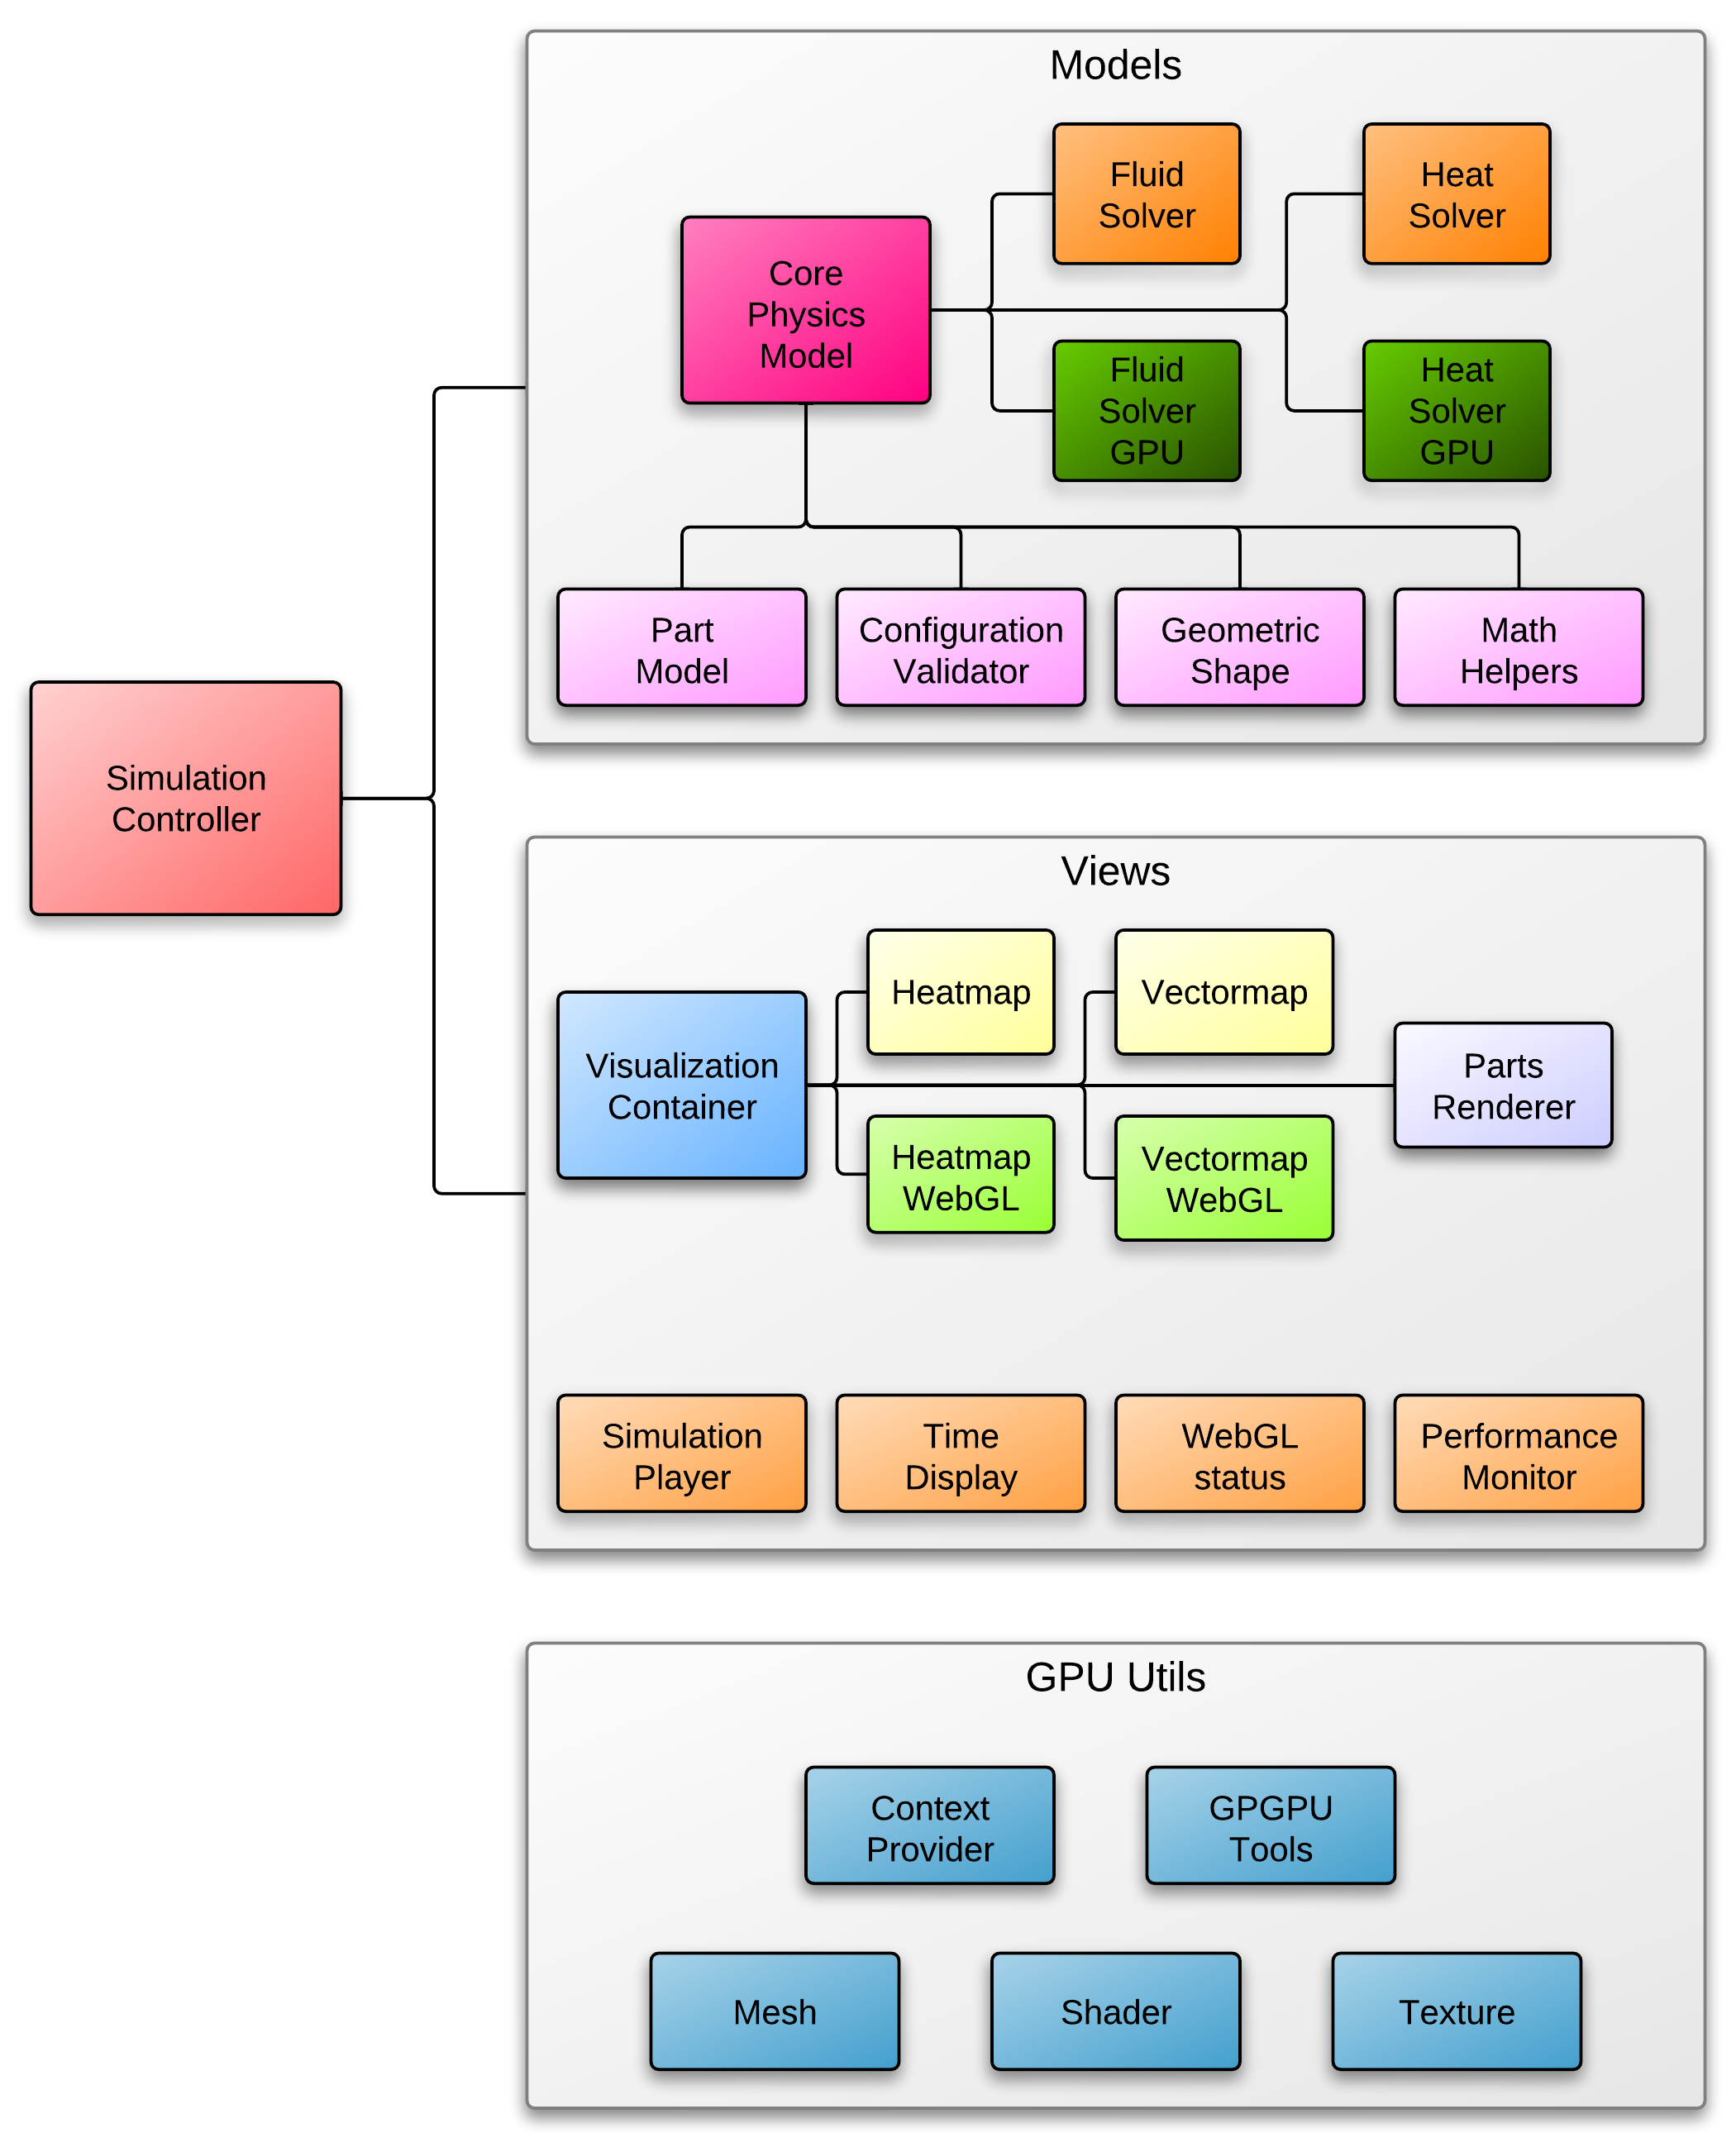
\includegraphics[width=\textwidth]{img/architektura}
\caption{Schemat ideowy architektury symulatora \en}
\label{fig:architektura}
\end{figure}

\section{Przegląd najistotniejszych jednostek symulatora}

W strukturze aplikacji można wyróżnić kilka wyraźnych grup charakteryzujących
się odmiennymi celami zasadniczymi. Wizualizacje tej struktury przedstawia
rysunek \ref{fig:architektura}, a kolejne sekcje przybliżają poszczególne grupy
oraz ich najważniejsze składniki.

\subsection{Modele}
\label{sec:modele}

Jest to zbiór obiektów odpowiedzialnych za przechowywanie i manipulowanie danymi
aplikacji. To właśnie w tej grupie znajdują się kluczowe dla całej aplikacji
silniki fizyczne odpowiadające za symulację przewodnictwa cieplnego oraz
dynamiki płynów.

\begin{description}

\item[Core Physics Model] tworzy i zarządza wszystkimi niezbędnymi dla obliczeń
fizycznych danymi. Można do nich zaliczyć siatki symulacyjne (reprezentowane
przez tablice \js bądź też dwuwymiarowe tekstury \ow{WebGL}) oraz zestaw
parametrów charakteryzujących warunki początkowe symulacji. Parametry te są
definiowane przez specjalny plik konfiguracyjny w formacie \ow{JSON}, dlatego
też można stworzyć bardzo wiele przypadków modelujących różnorakie zjawiska
fizyczne. Do zarządzania konfiguracją wykorzystywany jest jeden z pomocniczych
obiektów \textbf{Configration Validator}. Obliczenia fizyczne nie są
przeprowadzane przez sam obiekt \emph{Core Physics Model}. Deleguje on te
zadania do innych obiektów, tym samym realizując wzorzec projektowy strategii.

\item[Heat Solver oraz Fluid Solver] to obiekty implementujące algorytmy
fizyczne przewodnictwa cieplnego oraz dynamiki płynów przedstawione w sekcji
\ref{sec:silnikiFizyczne}. Implementacja została przeprowadzona wyłącznie w
języku \js dlatego też obliczenia wykonywane są na procesorze głównym
komputera.

\item[Heat Solver GPU oraz Fluid Solver GPU] to odpowiedniki obiektów
przedstawionych powyżej, jednak implementujące algorytmy fizyczne przy
wykorzystaniu technologii \ow{WebGL}. Stąd, główne obliczenia wykonywane są na
procesorze karty graficznej. Zapewnia to wielokrotnie lepszą wydajność.
Jednak, jako iż \ow{WebGL} jest technologią dość nową, obiekty te implementują
identyczną logikę jak wersje bazowe i są używane wyłącznie jeżeli konfiguracja
użytkownika spełnia odpowiednie wymagania.

\item[Part Model] to obiekt reprezentujący element symulacji nie będący płynem
(cieczą lub gazem). Dzięki obecności takich obiektów, możliwe jest stworzenie
ciekawych warunków początkowych odzwierciedlających rzeczywistość.  Zadaniem
elementów stałych symulacji jest tworzenie barier przepływu dla płynów. Ponadto
elementy stałe symulacji mogą przewodzić ciepło co dodatkowo wzbogaca symulacje
i pozwala zaprezentować np. efekt wpływu pojemności cieplnej na zdolność
przewodzenia ciepła.

\item[Geometric Shape oraz Math Helpers] to obiekty pomocnicze, wykorzystywane
głównie przez obiekty \emph{Part Model}. Definiują różne reguły matematyczne
pomocne przy reprezentowaniu i wizualizowaniu kształtów geometrycznych.

\end{description}

\subsection{Widoki}

Jest to zbiór obiektów odpowiedzialnych za aspekt wizualny symulacji. Ich
głównym zadaniem jest wizualizacja czyli prezentowanie przedstawionych powyżej
modeli. Przykładowy zrzut ekranu aplikacji \en wraz z zaznaczonymi obszarami
wygenerowanymi przez poszczególne widoki prezentuje rysunek \ref{fig:widoki}.

\begin{figure}[!h]
\centering
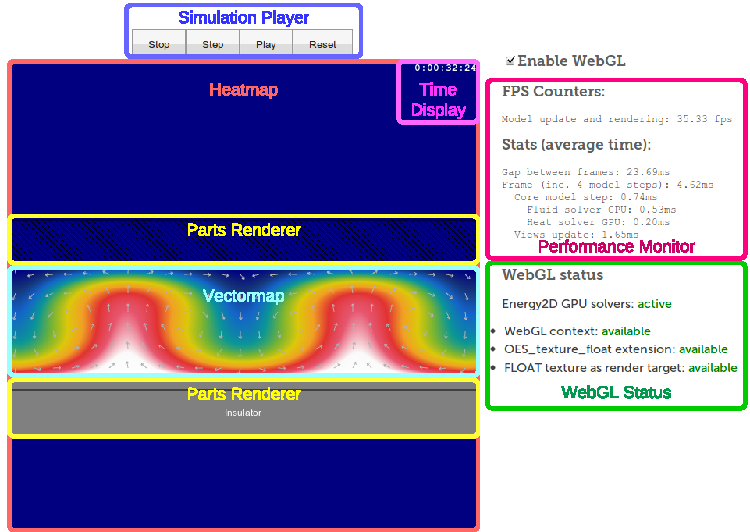
\includegraphics[width=\textwidth]{img/views}
\caption{Prezentacja poszczególnych widoków aplikacji \en}
\label{fig:widoki}
\end{figure}

\begin{description}

\item[Heatmap] to jeden z najważniejszych widoków, gdyż jest odpowiedzialny
za wizualizację temperatury. To dzięki temu możliwe jest obserwowanie zjawisk
zachodzących podczas symulacji. Wzorowany jest na obrazie kamer termowizyjnych.
Dostępnych jest także kilka palet kolorów.

\item[Vectormap] to widok odpowiedzialny za wyświetlanie strzałek prezentujących
prędkość i kierunek przepływu płynu. Umożliwia to lepsze zrozumienie zjawisk
prezentowanych podczas symulacji.

\item[Heatmap WebGL oraz Vectormap WebGL] to odpowiedniki powyższych widoków,
lecz korzystające z technologii \ow{WebGL}. Dzięki temu nie jest potrzebny
czasochłonny transfer danych z tekstury w pamięci karty graficznej do pamięci
głównej komputera.

\item[Parts Renderer] to widok mający za zadanie prezentacje elementów
stałych symulacji (czyli niebędących płynem).

\item[Visualization Container] to obiekt grupujący powyższe widoki, zapewniający
odpowiednie ich ułożenie oraz udostępniający pomocniczy interfejs do zarządzania
poszczególnymi podwidokami.

\item[Simulation Player] umożliwia sterowanie przebiegiem symulacji
(uruchomienie, zatrzymanie, odtwarzanie po jednym kroku, resetowanie do stanu
początkowego).

\item[WebGL Status] ma zadanie informacyjne, prezentuje czy konfiguracja
użytkownika wspiera technologię \ow{WebGL} oraz niezbędne jej rozszerzenia.

\item[Performance Monitor] prezentuje dane dotyczące wydajności, takie jak ilość
wyświetlanych klatek na sekundę oraz czasy wykonywania poszczególnych etapów
algorytmu. Dzięki niemu było możliwe przeprowadzenie testów wydajnościowych
omówionych w rozdziale \ref{sec:testyWydajnosciowe}.

\end{description}

\subsection{Kontroler}

Aplikacja \en definiuje tylko jeden kontroler -- \textbf{Simulation Controller}.
Jest on odpowiedzialny za wiele zadań, ale przede wszystkim stanowi spoiwo
łączące moduły odpowiedzialne za przeprowadzanie obliczeń fizycznych oraz moduły
odpowiedzialne za wizualizację. Zarządza relacjami między tymi obiektami oraz
steruje również przebiegiem symulacji.

\subsection{Narzędzia pomocnicze związane z GPU}

Podczas pracy nad optymalizacją polegającą na przeniesieniu obliczeń fizycznych
na GPU (por. rozdział \ref{cha:oblGPU}), pojawiła się potrzeba stworzenia
narzędzi, które stanowiłyby opakowanie dla niskopoziomowych funkcji API
\ow{WebGL}. 

\begin{description}

\item[Shader, Texture oraz Mesh] to obiekty przeznaczone do zarządzania
typowymi dla programowania grafiki trójwymiarowej strukturami -- odpowiednio:
programami jednostek cieniujących, teksturami oraz geometrią.

\item[GPGPU Tools] to moduł udostępniający zestaw funkcji ułatwiających
wykonywanie obliczeń ogólnego przeznaczenia na procesorze karty graficznej.
Jest głównie wykorzystywany przez obiekty takie jak \emph{Fluid Solver GPU}
oraz \emph{Heat Solver GPU}.

\end{description}


\section{Zgodność ze środowiskiem Node.js oraz przeglądarką internetową}
\label{sec:zgodNode.js}

\ow{Node.js}\footnote{Strona domowa projektu: \url{http://nodejs.org/}} to
dynamicznie rozwijające się środowisko \ow{JavaScript}, stworzone na bazie
silnika \ow{V8} opracowanego na potrzeby przeglądarki internetowej Google
Chrome. Aby skrypt mógł być wykonywany w tym środowisku, musi być niezależny od
cech charakterystycznych dla środowiska przeglądarki internetowej.

Niezależność od przeglądarki można zdefiniować jako niekorzystanie z metod
globalnie dostępnych obiektów takich jak \emph{window} czy też \emph{document}.
Innym działaniem, które wiąże skrypt z przeglądarką i tradycyjnym zastosowaniem
jest np. trawersowanie (oraz ewentualne modyfikowanie) drzewa HTML DOM. Jednak,
przy założeniu o niedostępności zewnętrznych bibliotek, można to sprowadzić do
nieużywania metod wspomnianego powyżej obiektu \emph{document}.

Poprzedni podrozdział zaprezentował modułową budowę symulatora \en na bazie
wzorca projektowego \emph{Model-View-Controller}. Architektura opierająca  się
na jak najbardziej niezależnych modułach, pełniących jasno zdefiniowaną funkcję
jest ważna nie tylko ze względu na łatwiejszy rozwój i utrzymanie aplikacji. To
podejście pozwoliło wyodrębnić jednostki symulatora, które są zupełnie
niezależne od przeglądarki wg. kryteriów zdefiniowanych powyżej. Warunek ten
spełnia grupa obiektów przedstawiona wcześniej jako ,,Modele'' (por.
\ref{sec:modele}). Dzięki niezależności od przeglądarki, możliwe stało się
używanie tych obiektów w przedstawionym powyżej środowisku \ow{Node.js}.

Główną korzyścią jaka z tego płynie jest możliwość stosowania wydajnych,
efektywnych testów zautomatyzowanych. Istnieją narzędzia umożliwiające
testowanie kodu \js związanego z przeglądarką, ale są to rozwiązania znacznie
mniej wydajne oraz wygodne. Oparcie testów na skryptach wykonywanych przez
\ow{Node.js} pozwoliło zintegrować testy z system ciągłej integracji \ow{Travis
Continuous Integration}\footnote{Strona domowa projektu: \url{http://travis-
ci.org/}}. Ponadto ułatwione zostało ewentualne użycie zaawansowanych silników
fizycznych \en przez inne aplikacje działające w środowisku \ow{Node.js}.

\section{Zarządzanie zależnościami w złożonych aplikacjach JavaScript}

Język \js natywnie nie wspiera żadnego mechanizmu zarządzania zależnościami. Nie
posiada instrukcji takich jak \emph{import} czy \emph{require}, znanych z innych
popularnych języków programowania, które pozwalają organizować źródła aplikacji.
W związku z tym twórcy aplikacji są zmuszeni rozwiązać ten problem
własnoręcznie. Najpopularniejsze podejścia do tego problemu to:

\begin{itemize}

\item Manualne zarządzanie zależnościami przez tagi \emph{<script>} bezpośrednio
w kodzie źródłowym strony HTML. Jest to rozwiązanie najprostsze jednak
programista jest zmuszony do ręcznego śledzenia zależności oraz zdefiniowania
skryptów w odpowiedniej kolejności. Z tego też powodu sprawdza się w praktyce
wyłącznie w małych, prostych aplikacjach.

\item Własne skrypty budujące aplikację, najczęściej poprzez zautomatyzowane
łączenie poszczególnych plików źródłowych w jeden plik wynikowy. Wykorzystywane
są do tego różne technologie. We wczesnym etapie rozwoju aplikacji \en właśnie
tak zarządzano zależnościami. Wykorzystywaną technologią był program
\emph{make}, dlatego pliki źródłowe zdefiniowane były w pliku \emph{Makefile}.
Podejście to jest znacznie lepsze niż poprzednie. Przede wszystkim pozwala
zbudować jeden wynikowy plik, który wystarczy dołączyć do strony HTML. Możliwe
staje się łatwe rozpowszechnianie aplikacji. Jednak wciąż programista musi
ręcznie śledzić i definiować zależności oraz zapewniać ich rozwiązywanie.

\item Technologie dedykowane. Niwelują one wady poprzednich podejść poprzez
automatyzacje całego procesu. Przykładem może być definicja modułów wg.
standardu CommonJS, używana np. w środowisku \ow{Node.js}. Innym standardem jest
AMD -- Asynchronous Module Definition. Potrzebne pliki źródłowe (moduły) są
wczytywane asynchronicznie, można też zadbać o to, żeby były dołączane wyłącznie
wtedy kiedy faktycznie są potrzebne. Implementacje tej technologii istnieją
zarówno dla przeglądarki jak i środowiska \ow{Node.js}. Dedykowane technologie
same rozwiązują zależności. Programista tylko je definiuje, dlatego też jest to
rozwiązanie korzystne (czasami wręcz niezbędne) w przypadku złożonych aplikacji.

\end{itemize}

W symulatorze \en wybrane zostało ostatnie z omówionych podejść. Zastosowano
implementację standardu AMD w postaci biblioteki RequireJS\footnote {Strona
domowa biblioteki: \url{http://requirejs.org/}}. Wybór samego podejścia jest
uzasadniony dużą złożonością aplikacji. Natomiast wybór tego konkretnego
standardu definicji modułów oraz biblioteki, która go implementuje podyktowany
był przede wszystkim zgodnością zarówno z przeglądarką internetową jak i
środowiskiem \ow{Node.js}.

\ow{RequireJS} posiada wiele alternatyw, jednak ta konkretna biblioteka jest
rozwijana i wspierana od długiego czasu, posiada ugruntowaną pozycję i rokuje
długie wsparcie w przyszłości. Definiowanie modułów odbywa się przez instrukcję
\emph{define} o następującej postaci:

\begin{lstlisting}[language=JavaScript, caption=Definicja modułu
przy użyciu technologii RequireJS]
define(['helper/utils', 'mymodule'], function (utils, mymodule) {
	var api = { /*...*/ };
	return api;
});
\end{lstlisting}

Dopuszczalna jest też alternatywna składnia, zbliżona do standardu CommonJS:

\begin{lstlisting}[language=JavaScript, caption=Alternatywna składnia definicji 
modułu przy użyciu technologii RequireJS]
define(function (require) {
	var utils 	 = require('helper/utils'),
		mymodule = require('mymodule'),
		api = { /*...*/ };
	return api;
});
\end{lstlisting}

Odpowiada ona dokładnie wersji podstawowej przedstawionej powyżej. W kodzie
\en jest używana najczęściej ze względu na subiektywne wrażenie większej
czytelności. Ponadto umożliwia bardzo łatwe konwertowanie modułów napisanych
pierwotnie w standardzie CommonJS, co również było użyteczne podczas pracy nad
aplikacją \en (gdyż pierwotnie silniki fizyczne były modułami zdefiniowanymi
właśnie w tym standardzie).


\chapter{Przeniesienie obliczeń fizycznych na procesor karty graficznej}

Niniejszy rozdział prezentuje techniki zastosowane w celu przeniesienia głównych
obliczeń fizycznych na kartę graficzną w symulatorze \ow{Energy2D} będącym
przedmiotem tej pracy. Na początku opisane są tradycyjne podejścia do tego
problemu dla aplikacji działających w natywnym środowisku systemu operacyjnego
oraz ich odniesienie do środowiska oferowanego przez przeglądarki internetowe.
Następnie zaprezentowane zostały najważniejsze zagadnienia dotyczące
implementacji równoległych silników fizycznych \ow{Energy2D} działających na
procesorze karty graficznej. Informacje te mogą być szczególnie użyteczne przy
próbach podobnych optymalizacji innych aplikacji.

Dzięki przeniesieniu obliczeń fizycznych na GPU uzyskano istotny wzrost
wydajności. Dokładna analiza zysków ze zrównoleglenia symulacji jest przedstawiona
w rozdziale \ref{cha:ocena}.

\section{Typowe metody przenoszenia obliczeń na GPU, a przeglądarka internetowa}

Współczesna karty graficzne posiadają ogromną moc obliczeniową -- wielokrotnie
większą od centralnego procesora przy założeniu, że obliczenia da się wykonywać
w sposób równoległy. Pomysł aby przenieść część obliczeń ogólnego zastosowania
na kartę graficzną pojawił się wraz z dynamicznym rozwojem procesorów
graficznych. Szczególnie istotnym momentem było wprowadzenie programowalnych
jednostek cieniujących (specyfikacja \ow{DirectX 8}). Dalszy rozwój obliczeń
ogólnego zastosowania na kartach graficznych (ang. \emph{General-Purpose
Computing on Graphics Processing Units}, w skrócie GPGPU) miał miejsce wraz z
wprowadzeniem technologii, które ukryły złożoność dostępu do zasobów karty
graficznej i udostępniły interfejs wysokiego poziomu. Wiodącymi technologiami
tego typu są \ow{OpenCL} (rozwiązanie otwarte) oraz \ow{CUDA} (zamknięte
rozwiązanie firmy NVIDIA, działające wyłącznie na sprzęcie tego producenta).

Wspomniane powyżej technologie dotyczą oczywiście aplikacji pisanych w natywnym
środowisku systemu operacyjnego. Aby programować jednostki cieniujące wystarczy
podstawowy dostęp do standardowego interfejsu \ow{OpenGL} bądź \ow{Direct3D}.
Implementacje tych interfejsów można znaleźć dla prawie każdego współczesnego
języka programowania. Interfejsy wyższego poziomu (\ow{OpenCL}, \ow{CUDA})
również posiadają implementacje w różnych językach programowania, choć
najczęstszym środowiskiem ich działania są aplikacje napisane w C bądź C++.

Poniżej krótko przedstawione są sposoby przeprowadzania obliczeń ogólnego
zastosowania na kartach graficznych oraz ich związek ze specyficznym
środowiskiem przeglądarki internetowej.

\subsection{Niskopoziomowe programowanie jednostek cieniujących}
\label{subsec:niskProgJedn}

Jest to najstarsze podejście do przeprowadzania obliczeń ogólnego zastosowania
na procesorze karty graficznej. Programista w swoisty sposób ,,oszukuje'' kartę
graficzną, przeprowadzając renderowanie prostej geometrii wyłącznie w celu
uruchomienia własnych programów jednostek cieniujących, które wykonują
obliczenia często nie mające nic wspólnego z generowaniem obrazu.

W przypadku technologii \ow{WebGL}, która posłużyła do zaimplementowania
silników fizycznych \en, diagram potoku renderowania prezentuje rysunek
\ref{fig:WebGLPipeline}. Zielonym kolorem zostały oznaczone procesy, które są
programowalne. Są to dwa rodzaje programów jednostek cieniujących --
wierzchołków oraz fragmentów. Nie ma możliwości bezpośredniego sterowania
pozostałymi procesami. Odbywają się one automatycznie, ewentualnie możliwa jest
konfiguracja pewnych parametrów. Dlatego też cały algorytm przeznaczony do
zrównoleglenia musi zostać zapisany wyłącznie przy użyciu programów wierzchołków
oraz fragmentów. Ponadto dane powinny się znajdować w pamięci karty graficznej,
najczęściej w postaci dwuwymiarowych tekstur.

\begin{figure}[!h]
\centering
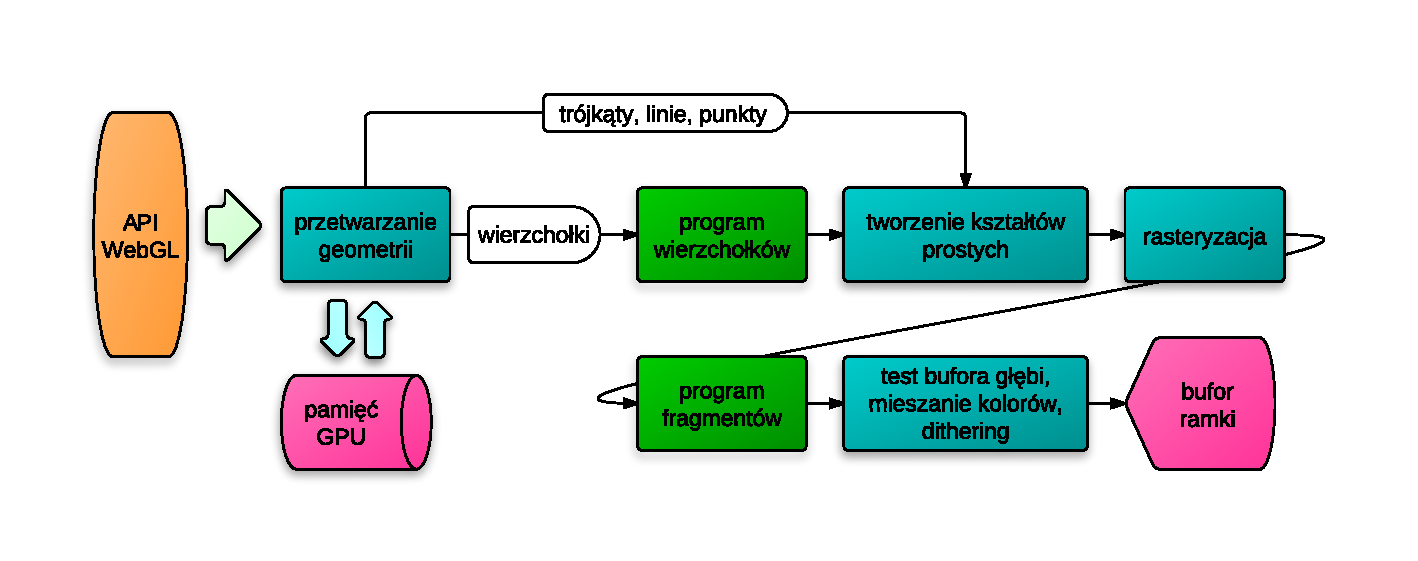
\includegraphics[width=\textwidth]{img/WebGLPipeline}
\caption{Diagram potoku renderowania \ow{WebGL} / \ow{OpenGL 3.x}}
\label{fig:WebGLPipeline}
\end{figure}

Takie podejście jednak jest wymagające i obarczone pewnymi problemami. Łatwo
popełnić błędy, wymagana jest też przynajmniej podstawowa wiedza o programowaniu
grafiki trójwymiarowej. Najważniejsze koncepcje niskopoziomowego programowania
jednostek cieniujących zostały doskonale przedstawione przez Marka Harrisa w
jednym z jego artykułów do popularnej serii \emph{GPU Gems} \cite{GPUConcepts}.

\subsection{Technologie wyższego poziomu}
\label{subsec:techWyzPoz}

Technologie, które przyczyniły się do gwałtownego wzrostu popularności obliczeń
na kartach graficznych to szczególnie \ow{OpenCL} oraz \ow{CUDA}.
Udostępniają  one znacznie wyższy poziom abstrakcji -- programista jest
zwolniony z obowiązku przyswojenia sobie niskopoziomowych mechanizmów rządzących
działaniem kart graficznych (choć ta wiedza pozwala tworzyć aplikacje
efektywniejsze). Udostępniony jest specjalny interfejs oraz składnia, co
znacznie ułatwia pracę, szczególnie programistom bez doświadczenia w pracy z
programowaniem grafiki trójwymiarowej.

\subsection{Możliwości w środowisku przeglądarki internetowej}
\label{subsec:srodPrzegInt}

Należy uściślić, że ,,środowisko przeglądarki internetowej'' to zbiór możliwości
nowoczesnych, wiodących przeglądarek internetowych, rozpowszechniony na tyle,
aby był dostępny dla większości użytkowników internetu. Równocześnie możliwości
te nie mogą wymagać instalowania żadnych dodatków i rozszerzeń, gdyż znacznie
ogranicza to ich dostępność. Jest to szczególnie istotne dla aplikacji
edukacyjnych, które wymagają łatwego i powszechnego dostępu.

Przeglądarka internetowa z założenia oferuje środowisko bardzo ograniczone,
przede wszystkim ze względów bezpieczeństwa. Jednak niedawno, wraz z nadejściem
standardu HTML5, został dodany podstawowy dostęp do zasobów karty graficznej.
Realizuje go technologia WebGL, która jest implementacją standardu \ow{OpenGL ES
2.0}. Tym samym pojawiła się możliwość programowania jednostek cieniujących kart
graficznych, a więc i przeprowadzania na nich obliczeń ogólnego zastosowania
(\ref{subsec:niskProgJedn}).

Technologie programowania kart graficznych wyższego poziomu
(\ref{subsec:techWyzPoz}) nie są (jeszcze) dostępne w przeglądarce internetowej.
Aktualnie trwają intensywne prace nad implementacją standardu OpenCL o roboczej
nazwie WebCL. Jednak technologia ta w aktualnym momencie jest na bardzo wczesnym
etapie rozwoju. Więcej informacji można znaleźć na stronie internetowej:
\url{http://www.khronos.org/webcl/}.

Dlatego też jedyną metodą na przeprowadzenie obliczeń ogólnego zastosowania na
procesorze karty graficznej w środowisku przeglądarki internetowej jest sposób
zaprezentowany w sekcji \ref{subsec:niskProgJedn}. Właśnie taka, niskopoziomowa
metoda została zastosowana dla silników fizycznych symulatora \ow{Energy2D}.
Opis najważniejszych zagadnień związanych z implementacją prezentuje następna
sekcja (\ref{sec:implSilFizWebGL}).

\section{Implementacji silników fizycznych Energy2D przy użyciu WebGL}
\label{sec:implSilFizWebGL}

Symulator \ow{Energy2D} składa się z dwóch kluczowych silników fizycznych -
przewodnictwa cieplnego oraz dynamiki płynów. Są one dokładnie przybliżone w
sekcji \ref{sec:silnikiFizyczne}. Oba te silniki są niezwykle wymagające
obliczeniowo. Dlatego też ich optymalizacja była zadaniem kluczowym, aby
stworzyć aplikację wartościową edukacyjnie. Zbyt wolny przebieg symulacji może
skutecznie zniechęcić większość potencjalnych użytkowników. Jednym z
podstawowych wymagań było, aby wirtualne laboratorium było aplikacją w pełni
interaktywną czyli również działającą jak najpłynniej.

Poniżej przedstawione są najważniejsze zagadnienia związanie z przeniesieniem
obliczeń fizycznych \ow{Energy2D} na kartę graficzną.

\subsection{Analiza algorytmów silników fizycznych pod kątem przetwarzania
równoległego}  

Wszystkie algorytmy rozwiązujące równania fizyczne w symulatorze \ow{Energy2D}
zostały poddane analizie pod kątem możliwości równoległego przetwarzania.
Zostały wyróżnione następujące kryteria, które algorytm musi spełniać, aby było
to możliwe:

\begin{itemize}

\item Możliwość reprezentowana danych w pamięci karty graficznej.

\item Niezależność wyniku algorytmu od sekwencji wykonywania obliczeń.

\end{itemize}

Jeżeli kryteria te są spełnione, powinna istnieć możliwość zaimplementowania
algorytmu w sposób równoległy. Oczywiście zmienia się strona techniczna, użyte
rozwiązania, język programowania oraz techniki, jednak sama koncepcja
algorytmu i główne kroki powinny pozostać bez większych zmian. Problem pojawia
się wtedy, gdy któryś z algorytmów nie spełnia jednego z tych kryteriów. W
takim przypadku konieczne są gruntowne modyfikacje lub rezygnacja z
implementacji takiego algorytmu.

Pierwszy warunek spełniają wszystkie algorytmy, jako że obliczenia są wykonywane
na prostokątnych siatkach symulacyjnych. Można je reprezentować w pamięci karty
graficznej przy użyciu dwuwymiarowych tekstur. Temat organizacji danych w
pamięci GPU oraz związane z tym problemy porusza sekcja \ref{sec:orgDanychWGPU}.

Drugi warunek nie został spełniony przez wszystkie zastosowane algorytmy.
Problematyczne okazały się metody rozwiązywania układów równań liniowych metodą
relaksacji \ow{Gaussa-Seidela} (por. \cite{GaussSeidel}). Podczas jednego
przebiegu przez wszystkie komórki macierzy, nowa wartość komórki $(i, j)$ jest
zależna od wartości komórek sąsiednich. Następnie komórka macierzy jest
niezwłocznie aktualizowana. Powoduje to, iż przy sekwencyjnym przetwarzaniu
wszystkich komórek, nowa wartość dla każdej komórki jest zależna od wartości
obliczonych zarówno w poprzednim kroku relaksacji jak i kroku aktualnym. W
sposób uproszczony schemat takiej relaksacji prezentuje algorytm
\ref{alg:GaussCPU}.

\begin{algorithm}[H]
  \caption{Relaksacja metodą Gaussa-Seidela na CPU}
  \label{alg:GaussCPU}
\begin{algorithmic}
\For {$0 \to relaxation\_steps$}
  \ForAll {$ \textrm{grid cells} $}
    \State $new\_val\gets f(x_{i,j}, x_{i+1,j}, x_{i-1,j}, x_{i,j+1}, x_{i,j-1})$
    \State $x_{i,j}\gets new\_val$
  \EndFor
\EndFor
\end{algorithmic}
\end{algorithm}

Niestety, przy obliczeniach równoległych nie można polegać na takiej zależności.
Każda komórka zostanie zaktualizowana na podstawie wartości komórek sąsiednich
wyłącznie z poprzedniego kroku relaksacji. Co więcej, ograniczeniem są też
kwestie czysto technologiczne - tekstury w których przechowywane są dane mogą
być podczas obliczeń wyłącznie przeznaczone do odczytu lub do zapisu. Tak więc
niemożliwy jest jednoczesny odczyt z danej tekstury oraz natychmiastowy zapis.

Problem ten został rozwiązany przez zmianę algorytmu rozwiązywania układów
równań liniowych na metodę relaksacji \ow{Jacobiego}. Główną różnicą jest moment
aktualizowania komórek siatki symulacji. W przeciwieństwie do metody \ow{Gaussa-
Seidela} nie następuje to natychmiast po obliczeniu nowej wartości dla danej
komórki, ale dopiero obliczeniu nowych wartości dla wszystkich komórek.
Uproszczony schemat tej relaksacji prezentuje algorytm \ref{alg:JacobiCPU}.

\begin{algorithm}[H]
  \caption{Relaksacja metodą Jacobiego na CPU}
  \label{alg:JacobiCPU}
\begin{algorithmic}
\For {$0 \to relaxation\_steps$}
  \ForAll {$ \textrm{grid cells} $}
    \State $temp_{i,j}\gets f(x_{i,j}, x_{i+1,j}, x_{i-1,j}, x_{i,j+1}, x_{i,j-1})$
  \EndFor
  \ForAll {$ \textrm{grid cells} $}
    \State $x_{i,j}\gets temp_{i,j}$
  \EndFor
\EndFor
\end{algorithmic}
\end{algorithm}

Taki algorytm można już przetworzyć na wersję równoległą. Macierze $x$ oraz
$temp$  zostają zamienione na odpowiednie tekstury. Również, w celach
wydajnościowych zawartość tekstur nie jest przepisywana tylko zamieniane są
ich referencje. Uproszczony schemat relaksacji metodą \ow{Jacobiego} na GPU
prezentuje algorytm \ref{alg:JacobiGPU}.

\begin{algorithm}[H]
  \caption{Relaksacja metodą Jacobiego na GPU}
  \label{alg:JacobiGPU}
\begin{algorithmic}
\For {$0 \to relaxation\_steps$}
  \ForAll {$ \textrm{grid cells} $} [IN PARALLEL]
    \State $temp_{i,j}\gets f(x_{i,j}, x_{i+1,j}, x_{i-1,j}, x_{i,j+1}, x_{i,j-1})$
  \EndFor
  \State swap $x$ with $temp$
\EndFor
\end{algorithmic}
\end{algorithm}

\begin{figure}[!p]
\centering

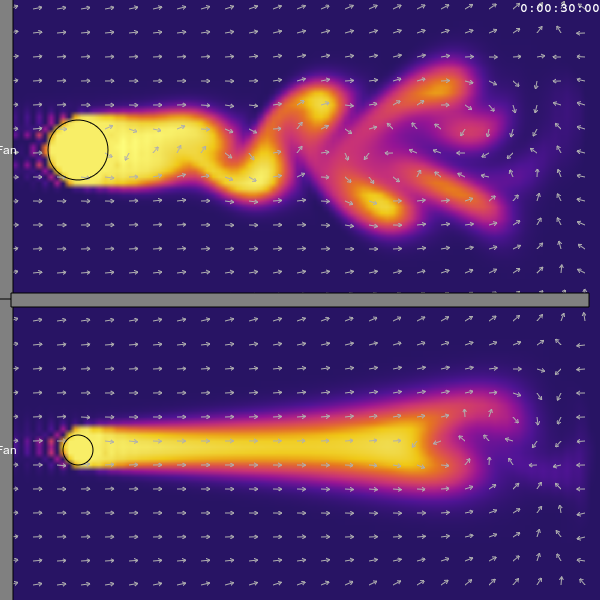
\includegraphics[width=.45\textwidth]{img/linSolvCPU5}
\caption{Symulacja przy użyciu metody Gaussa-Seidela na CPU, 
5 kroków relaksacji}
\label{fig:linSolvCPU5}

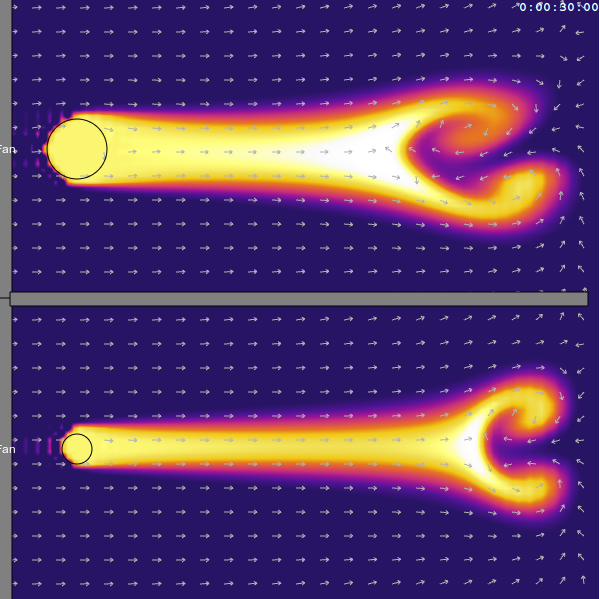
\includegraphics[width=.45\textwidth]{img/linSolvGPU5}
\caption{Symulacja przy użyciu metody Jacobiego na GPU, 
5 kroków relaksacji}
\label{fig:linSolvGPU5}

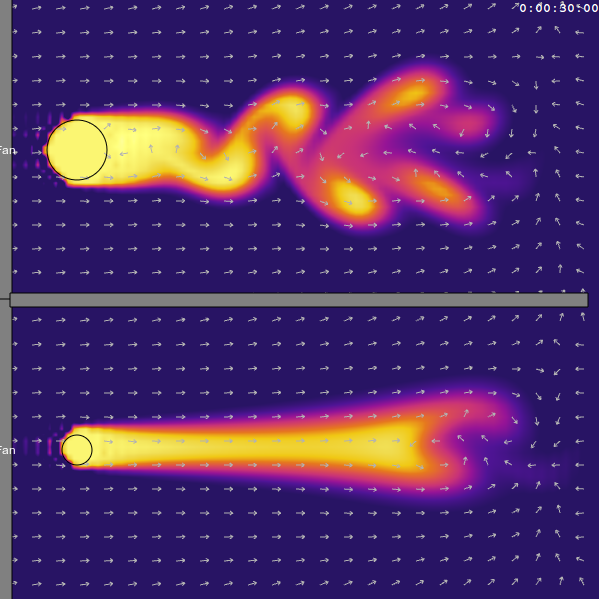
\includegraphics[width=.45\textwidth]{img/linSolvGPU10}
\caption{Symulacja przy użyciu metody Jacobiego na GPU, 
10 kroków relaksacji}
\label{fig:linSolvGPU10}

\end{figure}

Oczywiście zmiana algorytmu rozwiązywania równań liniowych niesie ze sobą
pewne konsekwencje. Inna jest konwergencja tych dwóch algorytmów. Metoda \ow
{Gaussa-Seidela} jest szybciej zbieżna niż metoda \ow{Jacobiego}. Efekty
symulacji dla różnej konfiguracji algorytmów rozwiązywania układów równań
liniowych prezentują rysunki \ref{fig:linSolvCPU5}, \ref{fig:linSolvGPU5} oraz
\ref{fig:linSolvGPU10}.

Na ww. rysunkach można zaobserwować wyraźne różnice w rezultatach symulacji. W
przypadku przedstawionej symulacji oczekiwanym wynikiem było powstane wiru
Kármána dla większej przeszkody. Przy implementacji równoległej metody
\ow{Jacobiego} widać, iż porządany efekt symulacji zostaje utracony. Dlatego
też należy wykonać więcej kroków relaksacji. Okazało się, że wartością
wystarczającą jest dziesięć. Wartość ta została ustalona empirycznie, tak aby
wyniki symulacji odpowiadały oczekiwaniom oraz były jak najbardziej zbliżone
do rezelutatów sekwencyjnych silików fizycznych. Jest to niezbędne, ponieważ
wersja równoległa aplikacji \en powinna być w pełni zgodnym i kompatybilnym
rozszerzeniem wersji podstawowej (sekwencyjnej, napisanej bez użycia
technologii \ow{WebGL}). Oczywiście wiąże się to ze spowolnieniem symulacji,
jednak w żadnym wypadku nie neguje opłacalności przeniesienia obliczeń na
kartę graficzną -- relaksacja na GPU jest wciąż dużo szybszych niż na CPU mimo
konieczności wykonania dwukrotnie większej liczby kroków.

Istnieją również implementacje algorytmu \ow{Gaussa-Seidela} na maszyny
równoległe. Nie są to dokładne kopie wersji sekwencyjnej, lecz imitują
obliczanie nowych wartości komórek na podstawie wartości z kroku relaksacji
poprzedniego i aktualnego. Doskonałe opracowanie zagadnień algorytmów
rozwiązujących układy równań liniowych na CPU oraz GPU, które okazało się
niezwykle przydatne podczas implementacji równoległych algorytmów dla \en,
zostało przygotowane przez G. Amadora oraz A. Gomesa \cite{LinSolvers}.
Niestety niskopoziomowa implementacja algorytmu \ow{Gaussa-Seidela} na GPU
wymaga wykonania dwóch procesów renderowania do tekstury dla jednego kroku
relaksacji -- powoduje to narzut czasowy, który w efekcie niweczy zysk z
szybszej konwergencji algorytmu.

\subsection{Podstawowy zarys implementacji}

Zgodnie z wnioskami sekcji \ref{subsec:srodPrzegInt}, ze względu na ograniczenia
środowiska przeglądarki internetowej, wymuszona została implementacja
niskopoziomowa przy użyciu technologii \ow{WebGL}. Opiera się ona na
programowaniu jednostek cieniujących karty graficznej, głównie wykorzystując
programy fragmentów (ang. fragment programs). Taka metoda przeprowadzania
obliczeń ogólnego przeznaczenia na karcie graficznej wymaga zrozumienia
podstawowych zagadnień związanych z programowaniem grafiki trójwymiarowej (por.
sekcja \ref{subsec:niskProgJedn}).

W przypadku implementacji \ow{Energy2D} podstawowy schemat przeprowadzania
obliczeń fizycznych na GPU z wykorzystaniem technologii \ow{WebGL} wygląda
następująco:

\begin{itemize}

\item Przygotowanie oraz kompilacja programów wierzchołków oraz fragmentów,
które zawierają implementację algorytmów silników fizycznych.

\item Przygotowanie tekstur, które przechowują dane symulacyjne. 

\item Przygotowanie danych geometrii płaszczyzny pokrywającej cały zakres
współrzędnych, które mieszczą się w obszarze renderowania.

\item Wykonywanie kolejnych kroków algorytmów fizycznych, co sprowadza się do:
	
	\begin{itemize}
	\item Renderowania wcześniej przygotowanej geometrii płaszczyzny przy użyciu
	wcześniej przygotowanych programów wierzchołków i fragmentów.

    \item Kopiowania danych z bufora ramki do wybranej tekstury przechowującej
	dane symulacji \footnote{Odbywa się to z użyciem obiektu bufora ramki (ang.
	FrameBuffer Object) z dołączoną do niego teksturą}.
	\end{itemize}

\end{itemize}

Poszczególne podpunkty w szerszym zakresie przybliżają sekcje od \ref{sec:progWierzFrag} do
\ref{sec:wykonNaGPU}.

\subsection{Programy wierzchołków oraz fragmentów}
\label{sec:progWierzFrag}

Właściwa implementacja algorytmów w programach wierzchołków i fragmentów
decyduje o poprawności oraz wydajności całej aplikacji. Bardzo często w
przypadku obliczeń ogólnego zastosowania na GPU, a także w przypadku
symulatora \ow{Energy2D}, większość pracy przypada na programy fragmentów.
Program wierzchołków zwykle sprowadza się do skopiowania wejściowych
współrzędnych wierzchołka i tekstury. Nie ma potrzeby jakiejkolwiek
modyfikacji geometrii renderowanej płaszczyzny. Dlatego też większość
programów wierzchołków w symulatorze Energy2D odpowiada poniższej
implementacji:

\begin{lstlisting}[language=GLSL, caption=Typowa implementacja programu
wierzchołków w symulatorze \ow{Energy2D} (język GLSL)]
attribute vec4 vertexPos;
attribute vec4 texCoord;

varying vec2 coord;
void main() {
  coord = texCoord;
  gl_Position = vertexPos;
}
\end{lstlisting}

Programy fragmentów, jako że wykonują właściwe obliczenia, nie są już tak
trywialne. Bardzo ważne jest właściwe określenie współrzędnych tekseli tekstury.
Posiadając siatkę symulacji o wymiarach NxN, należy ją zrzutować na zakres
domyślnych współrzędnych tekstury, które zawierają się w przedziale [0, 1].
Jeżeli zrobi się to nieprawidłowo, trudno będzie wykryć taki błąd, gdyż
domyślnie tekstury interpolują wartości leżące pomiędzy rzeczywistymi danymi.
Może to prowadzić do nieoczekiwanych rezultatów, stąd niezwykle istotne jest
precyzyjne określanie współrzędnych. W tym celu, praktycznie każdy program
fragmentów zawierał wektor o nazwie \ow{grid} równy (1.0 / N, 1.0 / N), gdzie
NxN to wymiary siatki symulacyjnej. Dodając lub odejmując odpowiedni jego
komponent można uzyskać dokładną wartość komórki sąsiedniej. Warto też pamiętać
o fakcie, iż pierwsza kolumna tekseli nie ma współrzędnej X równej 0.0, lecz 0.5
/ N. To samo dotyczy pierwszego rzędu współrzędnej Y równej 0.5 / N. Błędne
założenie, iż te kolumny mają współrzędne 0.0 prowadzi do problemów przy
wymuszaniu warunków brzegowych podczas symulacji. Ostatecznie, typowy szkielet
programów fragmentów wygląda następująco:

\begin{lstlisting}[language=GLSL, caption=Szkielet implementacji programu
fragmentów w symulatorze \ow{Energy2D} (język GLSL)]
uniform sampler2D simulationData;
uniform vec2 grid;
varying vec2 coord;

vec4 F(vec4 data) {
  // Funkcja wykonująca właściwe obliczenia dla danego kroku symulacji.
  // ...
}

void main() {
  vec4 data = texture2D(simulationData, coord);
  // Instrukcja warunkowa sprawdzająca czy nie są przetwarzane brzegi siatki.
  if (coord.x > grid.x && coord.x < 1.0 - grid.x &&
      coord.y > grid.y && coord.y < 1.0 - grid.y) {
    data = F(data);
  }
  gl_FragColor = data;
}
\end{lstlisting}

Oczywiście program, który wymuszał warunki brzegowe posiadał odwrotny warunek
w liniach 13 oraz 14. Implementacja funkcji $F$ nie jest przytoczona, gdyż nie
da się wyróżnić jakiegoś ogólnego jej schematu czy wzoru. Można powiedzieć, że
przenosząc dany krok algorytmu do języka GLSL, funkcja $F$ stanowi
implementację ,,wewnętrznych'' instrukcji zagnieżdżonych pętli iterujących po
wszystkich komórkach symulacji.


\subsection{Organizacja danych w pamięci karty graficznej}
\label{sec:orgDanychWGPU}
Dane symulacji (takie jak np. macierz temperatury czy macierz prędkości płynu)
przechowywane są w dwuwymiarowych teksturach zmiennoprzecinkowych. Tego typu
tekstury nie wchodzą w skład podstawowej specyfikacji \ow{WebGL 1.0}
(\cite{WebGLSpec}). W związku z tym wymagane jest użycie rozszerzenia
\ow{OES\_texture\_float}, które jest dostępne na większości
współczesnych urządzeń ([TODO: wspomnieć o rozdziale z testami]).

Niezwykle ważną kwestią jest organizacja danych w teksturze. Jest sporo
możliwości ponieważ tekstura z zasady nie jest wierną kopią tablicy JavaScript,
a obiektem przystosowanym do przechowywania obrazów (posiada na przykład kanały
kolorów). Dlatego też można rozważyć kilka potencjalnych sposobów na
rozmieszczenie danych.

\begin{itemize}

\item Schemat 1 -- tekstury jednokanałowe (format ALPHA lub LUMINANCE), jedna
tekstura odpowiada jednej tablicy JavaScript. Dalej nazywany schematem
\textbf{A1} na potrzeby niniejszego opracowania.

\item Schemat 2 -- tekstury czterokanałowe (format RGBA), dane tylko w jednym
kanale, jedna tekstura odpowiada jednej tablicy JavaScript. Dalej nazywany
schematem \textbf{RGBA1} na potrzeby niniejszego opracowania.

\item Schemat 3 -- tekstury czterokanałowe (format RGBA), dane w każdym z
kanałów, jedna tekstura odpowiada czterem tablicom JavaScript. Dalej nazywany
schematem \textbf{RGBA4} na potrzeby niniejszego opracowania.

\item Schemat 4 -- tekstury czterokanałowe (format RGBA), dane w każdym z
kanałów, jedna tekstura odpowiada jednej tablicy JavaScript, rozmiar tekstury
zredukowany czterokrotnie, gdyż każdy kanał odpowiada jednej ćwiartce tablicy.
Dalej nazywany schematem \textbf{RGBA1/4} na potrzeby niniejszego opracowania.

\end{itemize}

Każdy z powyższych schematów został przetestowany podczas implementacji
symulatora \ow{Energy2D}. Wyniki testów wydajnościowych przedstawia wykres
\ref{fig:texPerf}.

\begin{figure}[!h]
\centering
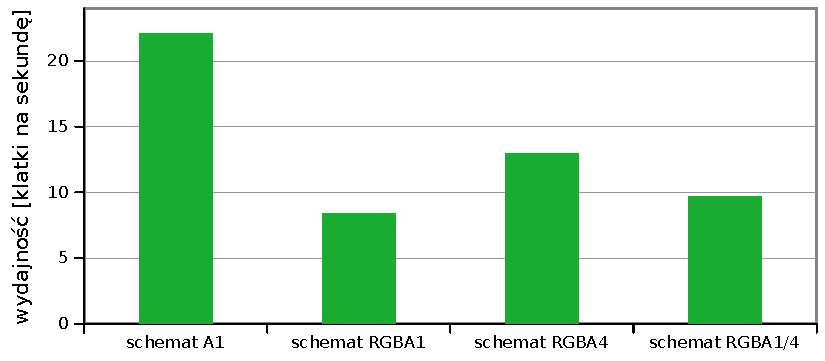
\includegraphics[width=.9\textwidth]{img/texPerf}
\caption{Wpływ organizacji danych w teksturach na wydajność symulacji 
\ow{Energy2D}}
\label{fig:texPerf}
\end{figure}

Rozwiązaniem optymalnym ze względu na wydajność oraz czytelność kodu wydaje się
schemat A1. Umożliwia on przeniesienie danych z tablic w relacji 1:1 do tekstur.
Do tego, każdy odczyt czy zapis do tekstury dotyczy tylko jednego kanału.
Niestety, na większości urządzeń nie ma możliwości dołączenia tekstury typu
ALPHA lub LUMINANCE do własnego obiektu bufora ramki (ang. FrameBuffer Object)
-- czyli renderowania do takiej tekstury \footnote{Testy zostały przeprowadzone
na systemie Linux (Ubuntu 12.04) i przeglądarce Google Chrome w wersji 22, która
korzysta z natywnego sterownika \ow{OpenGL}. Natomiast na tej samej konfiguracji
sprzętowej, ale działającej pod kontrolą systemu Windows nie udałoby się
uruchomić aplikacji. Podobnie w przypadku równie popularnego systemu
operacyjnego OS X.}. Wyklucza to możliwość użycia tego rozwiązania mimo
oczywistych zalet. Być może w przyszłości rozwój specyfikacji \ow{WebGL} na to
pozwoli.

Warto tutaj nadmienić, że specyfikacja \ow{WebGL} (\cite{WebGLSpec}) nie
gwarantuje, iż jakikolwiek z formatów tekstur zmiennoprzecinkowych będzie
zaakceptowany jako cel renderowania. Programista powinien wykonać test, aby
sprawdzić czy maszyna użytkownika wspiera daną konfigurację. Można to zrobić w
następujący sposób:

\begin{lstlisting}[language=JavaScript, caption=Weryfikacja poprawności formatu
i typu tekstury używanej jako cel renderowania]
var gl 		= getWebGLContext(),
	texture = gl.createTexture(),
	fbo 	= gl.createFramebuffer();

if (!gl.getExtension('OES_texture_float')) {
	throw new Error("Rozszerzenie OES_texture_float niedostępne.");
}
gl.bindTexture(gl.TEXTURE_2D, texture);
gl.texImage2D(gl.TEXTURE_2D, 0, gl.RGBA, 128, 128, 0, gl.RGBA, gl.FLOAT, null);
gl.bindFramebuffer(gl.FRAMEBUFFER, fbo);
gl.framebufferTexture2D(gl.FRAMEBUFFER, gl.COLOR_ATTACHMENT0, gl.TEXTURE_2D, texture, 0);
if (gl.checkFramebufferStatus(gl.FRAMEBUFFER) !== gl.FRAMEBUFFER_COMPLETE) {
	throw new Error("Dana tekstura nie jest wspierana jako cel renderowania.");
}
\end{lstlisting}

W praktyce tekstury zmiennoprzecinkowe posiadające cztery kanały kolorów są
najczęściej akceptowanym formatem do którego można zapisywać dane podczas
renderowania. Dlatego też schematy organizacji danych RGBA1, RGBA4 oraz RGBA1/4
używają takiego formatu tekstury.

Schemat RGBA1 posiada te same zalety co A1 jeśli chodzi o organizacje i
czytelność kodu źródłowego, jednak w tym przypadku dochodzi do dużego narzutu
wydajności związanego z odczytem i zapisem tekstur. Przy każdej z tych operacji
karta graficzna musi odczytać cztery kanały, jednak praktycznie wykorzystywany
jest tylko jeden z nich. Operacje dostępu do pamięci są czasochłonne, dlatego
też taka organizacja danych nie jest korzystna ze względów wydajnościowych.

Rozwiązaniem tego problemu są schematy RGBA4 oraz RGBA1/4. Organizacja danych
wg. trzeciego schematu pozwala zredukować narzut związany z odczytem oraz
zapisem pod warunkiem dobrej organizacji danych w teksturach. Pomysł ten
obrazuje diagram \ref{fig:rgba4Tex}. 

\begin{figure}[!h]
\centering
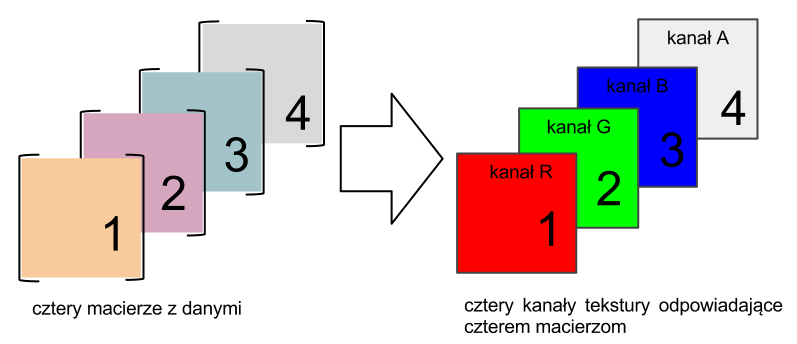
\includegraphics[width=.65\textwidth]{img/rgba4Tex}
\caption{Schemat organizacji danych z czterech macierzy w jednej teksturze}
\label{fig:rgba4Tex}
\end{figure}

Przy korzystnym ułożeniu danych jest możliwe praktycznie całkowite zredukowanie
narzutu związanego z odczytem wszystkich czterech kanałów tekstury, jednak w
praktyce jest to często niewykonalne. Przez korzystne rozmieszczenie danych
przyjmuje się takie ich ułożenie, żeby program jednostek cieniujących odczytując
teksturę faktycznie korzystał z danych zawartych w każdym z kanałów. Podobnie
przy zapisie, program renderujący powinien modyfikować wszystkie cztery kanały.
W przypadku symulatora \ow{Energy2D} udało się uzyskać taką organizację danych,
żeby odczyt był w znacznym stopniu zoptymalizowany, jednak podczas zapisu
modyfikowany był tylko jeden lub dwa kanały (kanał zawierający dane o
temperaturze lub kanały zawierające komponenty wektorów prędkości). Mimo nie do
końca optymalnego ułożenia kanałów, schemat RGBA4 okazał się wydajniejszy około
54\% od RGBA1.

\begin{figure}[!h]
\centering
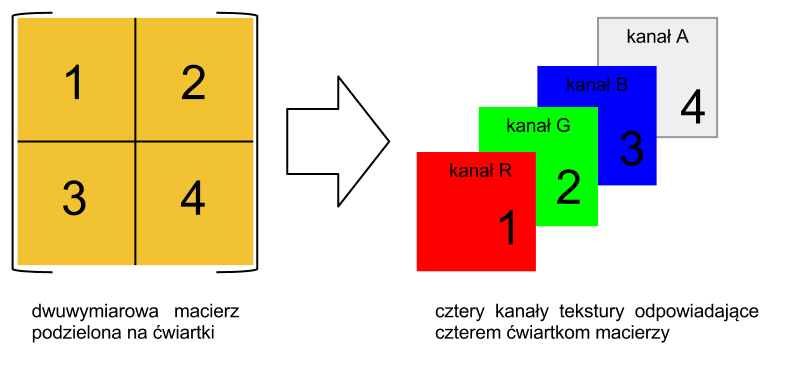
\includegraphics[width=.65\textwidth]{img/rgba14Tex}
\caption{Schemat organizacji danych macierzy NxN w teksturze (N/2)x(N/2)}
\label{fig:rgba14Tex}
\end{figure}

Ciekawą organizacją danych może wydawać się również pomysł przedstawiony w
schemacie RGBA1/4. Pozwala przechowywać tablicę JavaScript o wymiarach \ow{NxN}
w teksturze o wymiarach \ow{(N/2)x(N/2)}. Pomysł ten obrazuje diagram
\ref{fig:rgba14Tex}.

Taki układ danych teoretycznie posiada sporo zalet jak w przypadku użycia
tekstur jednokanałowych. Jednak znacznie zmniejsza on czytelność kodu i
komplikuje implementacje. Utrudnione zostaje przede wszystkim kontrolowanie
warunków brzegowych, programy jednostek cieniujących przetwarzają cztery pola
jednocześnie i stają się bardzo skomplikowane. W przypadku \ow{Energy2D}
komplikacje programów fragmentów były tak znaczne, że w efekcie odnotowano
bardzo słabe rezultaty pod względem wydajności. Symulacja okazała się być
wolniejsza około 34\% od symulacji korzystającej ze schematu RGBA4.

Dlatego też, ostatecznie w \ow{Energy2D} zastosowano schemat RGBA4. Zapewnia on
najlepszy kompromis pomiędzy dobrą wydajnością oraz wsparciem przez większość
dostępnych obecnie urządzeń.

\subsection{Geometria}

Podczas wykonywania obliczeń ogólnego przeznaczenia przy pomocy bezpośredniego
programowania jednostek cieniujących karty graficznej, niezbędne jest
stworzenie obiektu (a właściwie jego geometrii), który będzie renderowany. W
teorii może być to dowolna bryła. Jednak najczęściej pożądane jest, aby
program fragmentów wykonał się dla każdej komórki siatki symulacyjnej, którą
stanowi piksel tekstury. Można to osiągnąć renderując płaszczyznę, która
pokrywa całą dostępną przestrzeń renderowania.

Również w przypadku \en również wykorzystywany jest rendering takiej
płaszczyzny. Do przechowywania jej własności wykorzystane zostały bufory
wierzchołków (ang. vertex buffers) oraz indeksów (ang. index buffers)
znajdujące się w pamięci karty graficznej. Dzięki temu, podczas wielokrotnego
renderowania tej samej płaszczyzny, nie jest konieczne nieustanne przesyłanie
atrybutów wierzchołków do pamięci GPU.

W finalnej implementacji \en zostały przygotowane klasy pomocnicze
zarządzające geometrią oraz buforami. Jednak najprostszy sposób na stworzenie
płaszczyzny pokrywającej cały obszar renderowania oraz umieszczenie jej
atrybutów w pamięci karty graficznej zaprezentowany jest poniżej:

\begin{lstlisting}[language=JavaScript, caption=Definicja geometrii
płaszczyzny pokrywającej cały obszar renderowania]
var gl           = getWebGLContext(),
    vertexBuffer = gl.createBuffer(),
    indexBuffer  = gl.createBuffer(),
    vertexData,
    indexData;

// Współrzędne wierzchołków.
vertexData = new Float32Array([
    -1, -1, 
     1, -1,
    -1,  1,
     1,  1
]);
// Transfer do bufora wierzchołków.
gl.bindBuffer(gl.ARRAY_BUFFER, vertexBuffer);
gl.bufferData(gl.ARRAY_BUFFER, vertexData, gl.STATIC_DRAW);
// Indeksy trojkątów płaszczyzny.
indexData = new Uint16Array([
    0, 1, 2,
    2, 1, 3
]);
// Transfer do bufora indeksów.
gl.bindBuffer(gl.ELEMENT_ARRAY_BUFFER, indexBuffer);
gl.bufferData(gl.ELEMENT_ARRAY_BUFFER, indexData, gl.STATIC_DRAW);
\end{lstlisting}

\subsection{Wykonywanie kroków algorytmów na GPU}
\label{sec:wykonNaGPU}

Dysponując skompilowanymi programami wierzchołków oraz fragmentów, danymi
symulacji zapisanymi w teksturach dwuwymiarowych oraz niezbędną geometrią,
można przejść do faktycznej realizacji kroków algorytmów
zapisanych w programach jednostek cieniujących.

W przypadku technologii WebGL narzuca się schemat związany z techniką
renderowania do tekstury przy użyciu obiektu bufora ramki (ang. \emph{Frame
Buffer Object}). Związanie takiego obiektu z wybraną teksturą, a następnie
uaktywnienie przed właściwym renderowaniem, powoduje iż karta graficzna
automatycznie kopiuje zawartość bufora ramki do tekstury po zakończonym
renderowaniu.

Technika ta ma jednak kilka ograniczeń. Tekstura związana z obiektem bufora
ramki (czyli przeznaczona do zapisu) nie może być używana jednocześnie do
odczytu wartości. W związku z tym zawsze trzeba używać minimalnie jednej
tekstury tymczasowej. Następnie należy kopiować jej zawartość do tekstury
docelowej lub podmienić referencje. Oczywiście modyfikacja wyłącznie
referencji  jest znacznie efektywniejsza przez co i częściej stosowana.
Całościowo taki schemat nazywany jest ,,ping-pong rendering''.

Implementacja w języku \ow{JavaScript} przy użyciu technologi \ow{WebGL} nie
odbiega znacząco od implementacji w innych językach przy użyciu
,,tradycyjnego'' API OpenGL. Mark Harris zaprezentował najważniejsze aspekty
tej techniki w swoich artykułach opublikowanych w serii \emph{GPU Gems}
(\cite{GPUConcepts} oraz \cite{GPUFluid}).


\chapter{Ocena aplikacji}
\label{cha:ocena}

W tym rozdziale zaprezentowana została kompleksowa ocena aplikacji \en. Jest ona
podzielona na kilka części. Następnie zaprezentowane są testy jakościowe, które
opierają się na próbie odzwierciedlenia wybranych zjawisk fizycznych przy pomocy
symulatora. Z kolei testy wydajnościowe wersji podstawowej oraz równoległej \en
pokazują zysk jaki dało przeniesienie obliczeń na kartę graficzną. Na podstawie
tych wyników zanalizowana została dostępność aplikacji dla potencjalnych
użytkowników na różnych urządzeniach oraz ich konfiguracjach. Rozdział kończy
ocena stopnia realizacji założeń projektowych oraz krótkie podsumowanie.

\section{Modelowanie wybranych zjawisk fizycznych jako testy jakościowe symulatora}

W przypadku aplikacji edukacyjnej jaką jest symulator \en niezwykle istotne jest
aby symulowane zjawiska odzwierciedlały w sposób  wiarygodny rzeczywistość. Z
drugiej jednak strony, aplikacja musi być interaktywna i działać w czasie
rzeczywistym. Dlatego też nie można sobie pozwolić na zbyt długi czas
wykonywania, co zwykle idzie w parze z dokładnymi algorytmami i obliczeniami. Z
tego też powodu zastosowane silniki (algorytmy) fizyczne balansują pomiędzy
poprawnością fizyczną, a wydajnością (por. rozdział \ref{sec:silnikiFizyczne}).
Jest to dopuszczalne, ponieważ symulacja jest zorientowana wyłącznie na aspekt
wizualny.

Z powodu tego kompromisowego podejścia do pełnej dokładności obliczeń, niezwykle
istotne były testy aplikacji pod kątem podstawowej poprawności fizycznej. W tym
celu zostały przygotowane przypadki testowe, które miały za zadanie modelować
powszechnie znane zjawiska fizyczne związane z przewodnictwem cieplnym oraz
dynamiką płynów. Poniżej przedstawione są wyniki tych testów.

\subsection{Komórki Bénarda}

Modelowanie komórek Bénarda to jeden z podstawowych testów aplikacji
symulujących dynamikę płynów. Są to komórki konwekcyjne powstające w płynie
podgrzewanym od spodu. Rysunek \ref{fig:physBenard} prezentuje wyniki symulacji
przeprowadzonej przez \en.

\begin{figure}[!h]
\centering
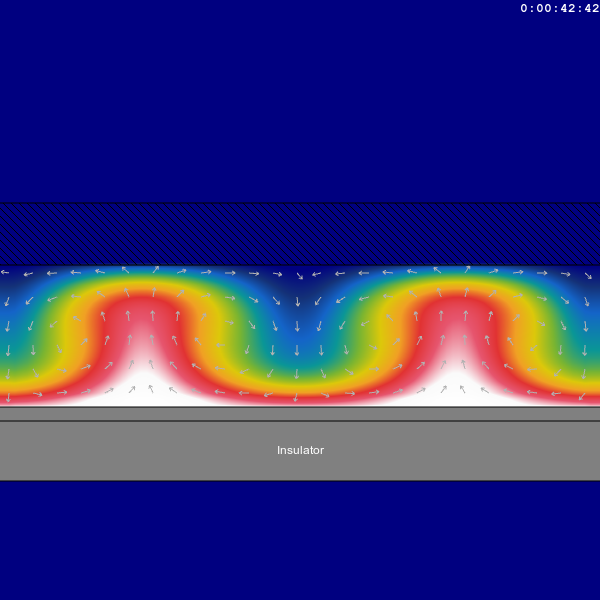
\includegraphics[width=0.8\textwidth]{img/physics/benard}
\caption{Symulacja formowania się komórek Bénarda}
\label{fig:physBenard}
\end{figure}

Wyraźnie widać formowanie się oczekiwanych komórek. Ich układ oraz kształt
stabilizuje się po bardzo krótkim czasie symulacji. Wyniki można uznać za w
pełni satysfakcjonujące.

\subsection{Przepływ laminarny oraz turbulentny}
\label{sec:przeplywyLamTur}

Symulacja przepływów laminarnych oraz turbulentnych to następny test silnika
dynamiki płynów. Rodzaj przepływu, w przypadku gdy jest on zakłócony przez
obecność przeszkody, w głównym stopniu determinuje liczba Reynoldsa. Jest ona
zależna od:

\begin{itemize}
\item lepkości płynu,
\item prędkości przepływu,
\item średnicy przeszkody.
\end{itemize}

W związku z tym został przygotowany przypadek testowy, w którym płyn ma stałą
lepkość, a przeszkody identyczne wymiary. Zmienna jest tylko prędkość przepływu.
Dla mniejszych prędkości oczekiwanym wynikiem był przepływ laminarny, dla
większych przepływ turbulentny. Rysunek \ref{fig:physLaminarTurbulent}
prezentuje wyniki takiej symulacji przeprowadzonej przez \en.

\begin{figure}[!h]
\centering
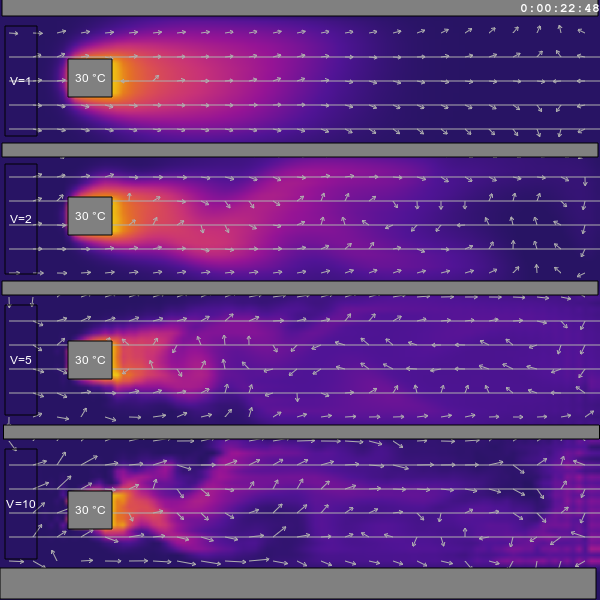
\includegraphics[width=0.8\textwidth]{img/physics/laminarTurbulent}
\caption{Symulacja wpływu liczby Reynoldsa na rodzaj przepływu}
\label{fig:physLaminarTurbulent}
\end{figure}

Rezultaty są zgodne z oczekiwaniami. Wyraźnie widać wpływ liczby Reynoldsa
(determinowanej przez prędkość płynu) na rodzaj przepływu.

\subsection{Ścieżka wirowa von Kármána}

Ścieżka wirowa von Kármána to kolejny doskonały test silnika dynamiki płynów.
Jest to szczególny rodzaj przepływu turbulentnego, który powstaje wyłącznie dla
pewnego zakresu wartości liczby Reyonldsa (por. \ref{sec:przeplywyLamTur}).

W związku z tym został przygotowany przypadek testowy, w którym płyn ma stałą
lepkość oraz prędkość przepływu, natomiast zmienna jest tylko średnica
przeszkody. Zgodnie z powyższymi założeniami, powinno być możliwe dobranie
takich średnic przeszkód, aby wiry Kármána powstały tylko za większą z nich.
Rysunek \ref{fig:physKarman} prezentuje wyniki takiej symulacji przeprowadzonej
przez \en.

\begin{figure}[!h]
\centering
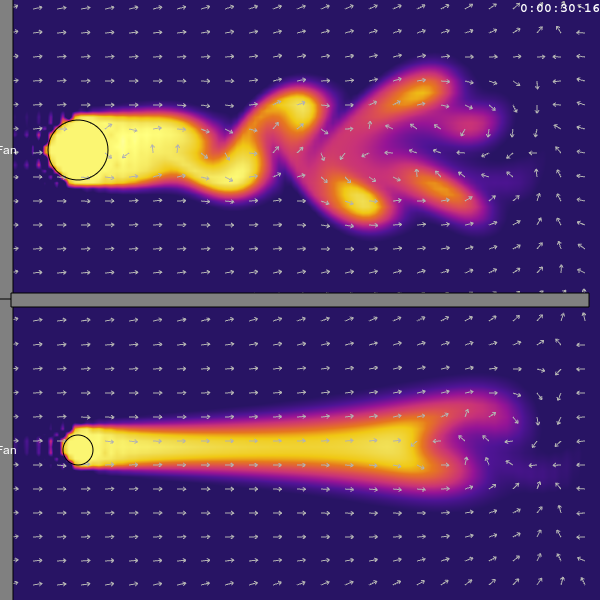
\includegraphics[width=0.8\textwidth]{img/physics/karman}
\caption{Symulacja formowania się wirów Kármána}
\label{fig:physKarman}
\end{figure}

Rezultaty są zgodne z oczekiwaniami. Wir powstał tylko w warunkach, w których
liczba Reynoldsa była większa.

\subsection{Pojemność cieplna}

Tym razem przypadek testowy dotyczy silnika przewodnictwa cieplnego. Pojemność
cieplna jest wielkość fizyczna, która charakteryzuje ilość ciepła, jaka jest
niezbędna do zmiany temperatury ciała o jednostkę temperatury. Poprawna
symulacja powinna uwzględniać ten parametr materiałów.

Aby to sprawdzić przygotowany został przypadek testowy, w którym znajdują się
dwa materiały o różnej pojemności cieplnej. Materiał o większej pojemności
powinien przewodzić ciepło znacznie lepiej niż ten o pojemności mniejszej.
Wyniki takiego eksperymentu przeprowadzonego przez symulator \en prezentuje
rysunek \ref{fig:heatCapacity}.

\begin{figure}[!h]
\centering
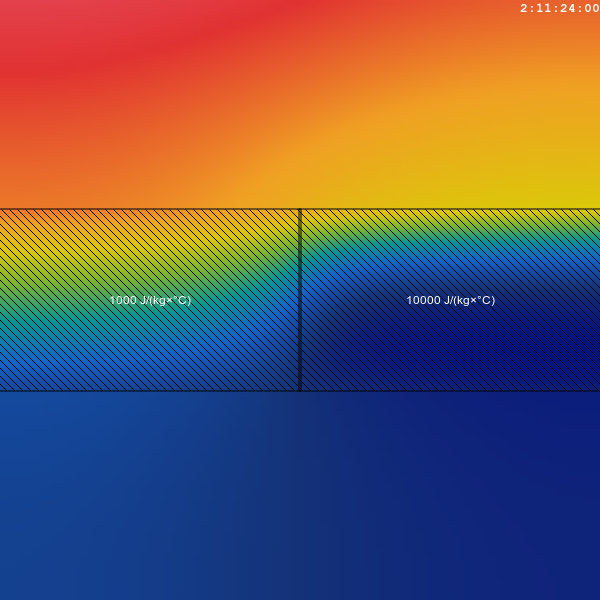
\includegraphics[width=0.8\textwidth]{img/physics/heatCapacity}
\caption{Symulacja wpływu pojemności cieplnej na przewodnictwo cieplne}
\label{fig:heatCapacity}
\end{figure}

Rezultaty po raz kolejny są zgodne z oczekiwaniami. Widać wyraźnie, iż materiał
o większej pojemności cieplnej znacznie lepiej przewodzi ciepło.

\subsection{Aspekt edukacyjny}

Ostatni z zaprezentowanych testów jest bardziej złożony. Nie prezentuje on
jednego, konkretnego zjawiska fizycznego jak poprzednie przykłady. Skupia się on
na zaprezentowaniu przykładowych możliwości symulacji oraz na potencjalnym
aspekcie edukacyjnym.

Przygotowana została scena zawierająca nieszczelnie izolowane pomieszczenie,
będące metaforą mieszkania. Jest ono ogrzewane przez element grzewczy o stałej
mocy. W jego otoczeniu został wymuszony dość mocny przepływ symulujący wiatr.
Miało to na celu pokazanie użytkownikom różnych, potencjalnych dróg ucieczki
ciepła z pomieszczeń mieszkalnych.

\begin{figure}[!h]
\centering
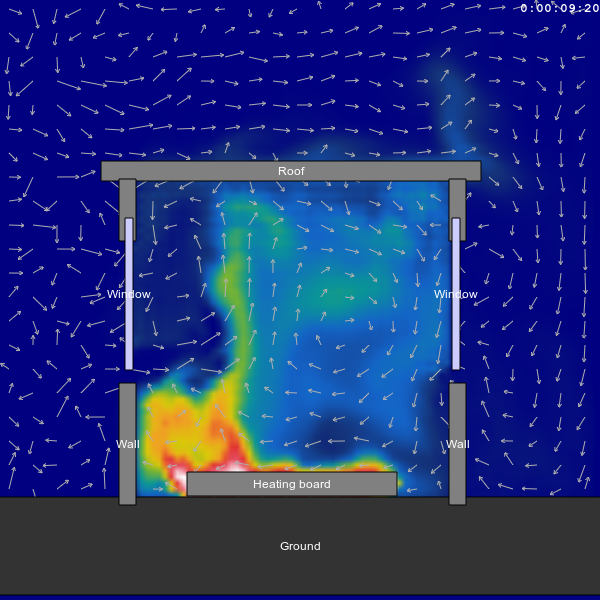
\includegraphics[width=0.8\textwidth]{img/physics/wind}
\caption{Symulacja ucieczki ciepła z pomieszczeń mieszkalnych}
\label{fig:wind}
\end{figure}

Rysunek \ref{fig:wind} prezentuje efekty takiej symulacji. Widoczne są dwa
wyraźne zjawiska -- strata ciepła w okolicy nieszczelnych okien oraz strata
ciepła związana z przewodnictwem cieplnym dachu. Pozwala to lepiej zrozumieć
użytkownikowi (docelowo uczniowi na początkowym etapie edukacji) wpływ różnych
aspektów pomieszczeń mieszkalnych (takich jak szczelność czy izolacja) na straty
ciepła. Może przyczynić się to do rozsądniejszego i ekonomiczniejszego
gospodarowania energią w jego własnym mieszkaniu czy też domu. W dobie
szczególnej dbałości o środowisko naturalne jest to niezwykle cenny i pożądany
efekt edukacyjny.

\section{Testy wydajnościowe}

Wydajność jest kluczowym aspektem symulacji ukierunkowanej na cele edukacyjne.
Tylko odpowiednia prędkość symulacji może przyciągnąć uwagę użytkownika i
zachęcić go do dalszej eksploracji zagadnienia.

W celu osiągnięcia zadowalającej wydajności na różnych urządzeniach zastosowano
kilka technik. Podstawową jest świadoma implementacja polegająca na unikaniu
zbędnych, czasochłonnych operacji, wynikająca ze znajomości środowiska
przeglądarki internetowej. Jednak krokiem, który najbardziej przyczynił się do
powstania naprawdę wydajnej aplikacji było przeniesienie obliczeń związanych
z fizyką na procesor karty graficznej.

Niniejsza sekcja przedstawia zyski z zastosowania tej optymalizacji. Omówiona
jest także kwestia wpływu konfiguracji sprzętowej użytkownika oraz związana z
tym ogólna dostępność symulatora dla szerokiego grona odbiorców.

\subsection{Metodologia testów}

Za wyznacznik wydajności została przyjęta liczba klatek na sekundę animacji,
którą jest w stanie generować działająca aplikacja \en. Jedna klatka domyślnie
składa się z:

\begin{itemize}
\item czterech kroków symulacji, 
\item odświeżenie wizualizacji.
\end{itemize}

Takie też ustawienia zostały zastosowane podczas wszystkich testów. 

Aplikacja wymusza kolejne klatki poprzez użycie metody \ow{setInterval()} z
czasem 0. Powoduje to, iż przeglądarka nie wprowadzi żadnych dodatkowych
opóźnień między klatkami i przejdzie do generowania kolejnej natychmiast, gdy
będzie to możliwe. Nie została użyta zalecana w przypadku aplikacji
\ow{WebGL}funkcja \ow{requestAnimationFrame()}, ponieważ wprowadza ona limit 60
klatek na sekundę i koncentruje się na utrzymaniu stałego tempa animacji, a nie
osiągnięciu maksymalnej wydajności. Zaburzało to w istotny sposób wiarygodność
wyników.

Na potrzeby testów zostały przygotowane specjalne przypadki testowe. Różnią się
one między sobą:
\begin{itemize} 
\item układem sceny, 
\item modelowanym zjawiskiem fizyczny,
\item użytymi silnikami fizycznymi:
	\begin{itemize} 
	\item wyłącznie silnik przewodnictwa cieplnego,
	\item silnik przewodnictwa cieplnego oraz silnik dynamiki płynów,
	\end{itemize}
\item rozmiarem siatki symulacyjnej.
\end{itemize}

Tabela \ref{tab:przypTest} prezentuje symboliczne nazwy przypadków testowych
wraz z ich krótką charakterystyką. Skrót HT pochodzi od ang. Heat Transfer i
oznacza, że dany przypadek testowy korzysta z silnika przewodnictwa cieplnego. Z
kolei skrót CDF pochodzi od ang. Computational Fluid Dynamics i oznacza, że dany
przypadek testowy korzysta z silnika dynamiki płynów. Wizualizację symulacji
przypadków testowych prezentują rysunki \ref{fig:ht1}, \ref{fig:ht2},
\ref{fig:cfd1} oraz \ref{fig:cfd2}.


\begin{table}
\caption{Zestawienie charakterystyki przypadków testowych do pomiaru wydajności}
\centering
\begin{tabular}{|l|c|c|c|l|}
\hline
nazwa testu & siatka & HT & CFD & opis \\ \hline
\textbf{ht1-100} & $100x100$ & \checkmark & $\times$ &
symulacja przewodnictwa cieplnego \\ \hline

\textbf{ht1-512} & $512x512$ & \checkmark & $\times$ &
symulacja przewodnictwa cieplnego \\ \hline

\textbf{ht1-1024} & $1024x1024$ & \checkmark & $\times$ &
symulacja przewodnictwa cieplnego \\ \hline

\textbf{ht2-100} & $100x100$ & \checkmark & $\times$ &
symulacja przewodnictwa cieplnego \\ \hline

\textbf{ht2-512} & $512x512$ & \checkmark & $\times$ &
symulacja przewodnictwa cieplnego \\ \hline

\textbf{ht2-1024} & $1024x1024$ & \checkmark & $\times$ &
symulacja przewodnictwa cieplnego \\ 

\hline \hline 

\textbf{cfd1-100} & $100x100$ & \checkmark & \checkmark &
symulacja dynamiki płynów \\ \hline

\textbf{cfd1-256} & $256x256$ & \checkmark & \checkmark &
symulacja dynamiki płynów \\ \hline

\textbf{cfd2-100} & $100x100$ & \checkmark & \checkmark &
symulacja dynamiki płynów \\ \hline

\textbf{cfd2-256} & $256x256$ & \checkmark & \checkmark &
symulacja dynamiki płynów \\ \hline
\end{tabular}

\label{tab:przypTest}
\end{table}

\begin{figure}[!p]
\begin{minipage}[b]{0.47\linewidth}
\centering
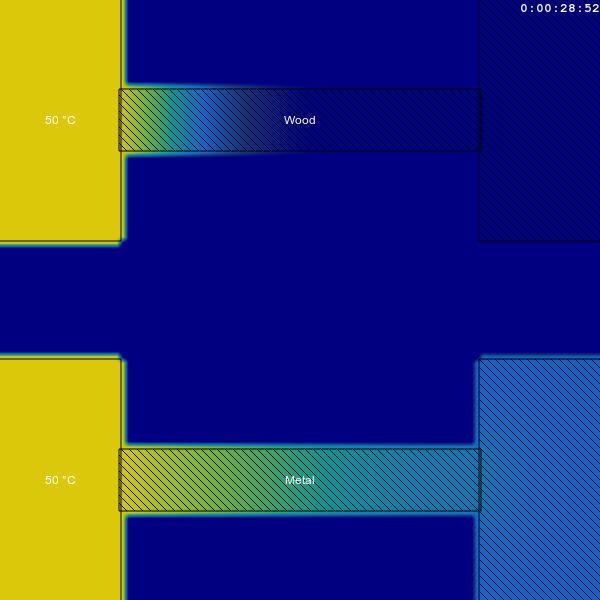
\includegraphics[width=\textwidth]{img/perfCase/ht1}
\caption{Symulacja ht1-100/512/1024}
\label{fig:ht1}
\end{minipage}
\hspace{0.04\linewidth}
\begin{minipage}[b]{0.47\linewidth}
\centering
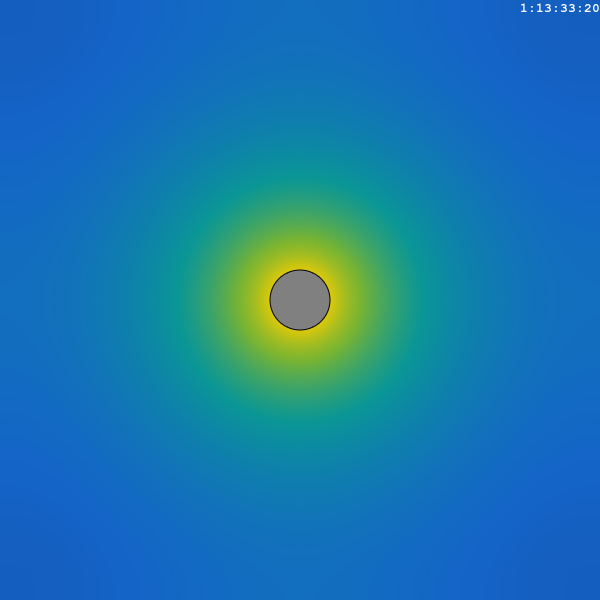
\includegraphics[width=\textwidth]{img/perfCase/ht2}
\caption{Symulacja ht2-100/512/1024}
\label{fig:ht2}
\end{minipage}
\end{figure}
\begin{figure}[!p]
\begin{minipage}[b]{0.47\linewidth}
\centering
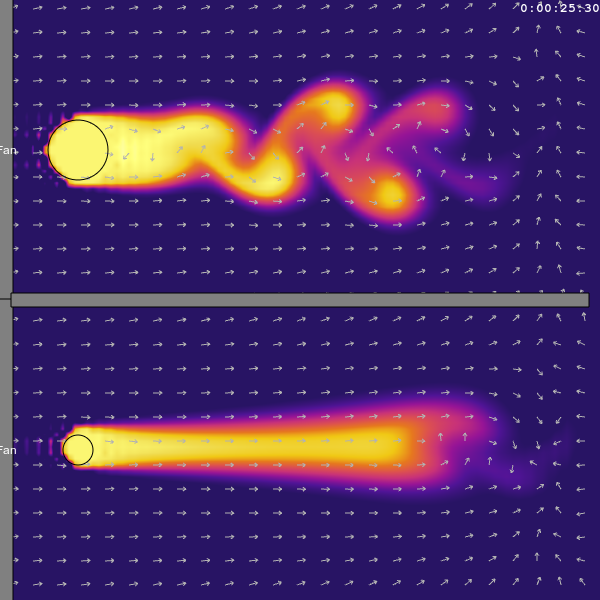
\includegraphics[width=\textwidth]{img/perfCase/cfd1}
\caption{Symulacja cfd1-100/256}
\label{fig:cfd1}
\end{minipage}
\hspace{0.04\linewidth}
\begin{minipage}[b]{0.47\linewidth}
\centering
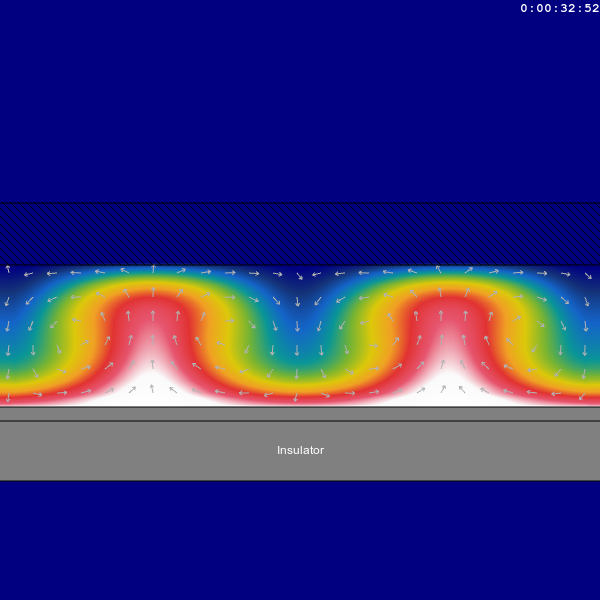
\includegraphics[width=\textwidth]{img/perfCase/cfd2}
\caption{Symulacja cfd2-100/256}
\label{fig:cfd2}
\end{minipage}
\end{figure}

\subsection{Konfiguracje sprzętowe przeznaczone do testów}

Testy zostały przeprowadzone na następujących komputerach:

\begin{itemize}

\item laptop Samsung QX510,
\item laptop Apple MacBook Pro, wersja z roku 2010,
\item laptop Apple MacBook Pro, wersja z roku 2012,
\item komputer stacjonarny.

\end{itemize}

\begin{table}[!h]
\caption{Charakterystyka komputerów testowych}
\centering
\begin{tabular}{|l|l|l|l|}
\hline
nazwa & procesor & karta graficzna & system operacyjny \\ \hline
Samsung QX510 & Intel Core i5 2.66GHz & NVIDIA GT 420M & Ubuntu 12.04 \\ \hline
MacBook Pro 2010 & Intel Core i7 2.66GHz & NVIDIA GT 330M & Mac OS X 10.6.8 \\ \hline
MacBook Pro 2012 & Intel Core i7 2.3GHz & NVIDIA GT 650M & Mac OS X 10.7.4 \\ \hline
stacjonarny & Intel Core2Quad 2.5GHz & NVIDIA 9600GT & Windows 7 \\ \hline
\end{tabular}
\label{tab:komputery}
\end{table}

Ich dokładną specyfikację prezentuje tabela \ref{tab:komputery}.
Konfiguracje znacznie różnią się od siebie. Działają pod kontrolą trzech
najpopularniejszych systemów operacyjnych -- Linux (Ubuntu), Mac OS X oraz
Windows 7. Również moc obliczeniowa kart graficznych jest bardzo zróżnicowana.

\subsection{Porównanie wydajności w różnych przeglądarkach internetowych}

Aplikacja od początku rozwoju była głównie testowana w przeglądarce Google
Chrome, gdyż wyraźnie było widać jej ogromną przewagę w kwestii wydajności
silnika \ow{JavaScript}. Ponadto, wg. ostatnich raportów, jest to
najpopularniejsza przeglądarka na świecie, tak więc potencjalnie najwięcej
użytkowników \en będzie z niej korzystać. Raport \cite{BrowserStats} pokazuję,
iż w lipcu 2012 roku z przeglądarki Google Chrome korzystało 42.9\% użytkowników
internetu. Drugie miejsce należało do przeglądarki Mozilla Firefox z udziałem
33.7\%. Łącznie te dwie przeglądarki posiadają 77.6\% ,,rynku'', dlatego są
traktowane priorytetowo. Kolejna popularna przeglądarka Internet Explorer
została wyłączona z testów z powodu niedostępności poza środowiskiem Windows
oraz braku wsparcia dla technologii \ow{WebGL}. Podobnie Safari, które wspiera
\ow{WebGL} jednak działa tylko na systemie operacyjnym Mac OS. Dlatego też testy
zostały przeprowadzone wyłącznie z użyciem następujących przeglądarek:

\begin{itemize}
\item Google Chrome v. 22
\item Mozilla Firefox v. 16
\item Opera v. 12.50
\end{itemize}

Środowiskiem testowym był laptop Samsung QX510 (por. tablica \ref{tab:komputery}).

\subsubsection{Obliczenia fizyczne wykonywane na CPU}

Wyniki pomiarów wydajności symulatora w przypadku obliczeń przeprowadzanych na
CPU prezentuje tabela \ref{tab:przegladarki} oraz wykres \ref{fig:browserPerf}.
Nietrudno dostrzec ogromną przewagę przeglądarki Google Chrome. Jest to efekt
zastosowanego w niej niezwykle wydajnego silnika \ow{JavaScript} o nazwie V8.
Opera oraz Mozilla Firefox posiadają zbliżoną wydajność, jednak Opera jest
nieznacznie szybsza. Warto też zauważyć, iż kiedy obliczenia fizyczne
przeprowadzane są na CPU, jedyną przeglądarką, która zapewnia odpowiednią
prędkość wykonywania się symulacji jest Google Chrome.

\begin{table}[!h]
\caption{Wydajność symulacji na CPU w zależności od przeglądarki}
\centering
\begin{tabular}{|c|p{3cm}|p{3cm}|p{3cm}|}
\hline
test & Google Chrome & Mozilla Firefox & Opera \\ \hline
ht1-100 & 45.20 & 11.12 & 11.83 \\ \hline
h1-512 & 3.24 & 0.45 & 0.98 \\ \hline
ht1-1024 & 0.92 & 0.11 & 0.25 \\ \hline
ht2-100 & 48.04 & 10.73 & 12.05 \\ \hline
ht2-512 & 3.34 & 0.40 & 0.84 \\ \hline
ht2-1024 & 0.89 & 0.11 & 0.22 \\ \hline
cfd1-100 & 22.25 & 2.51 & 3.84 \\ \hline
cfd1-256 & 4.24 & 0.38 & 0.93 \\ \hline
cfd2-100 & 20.60 & 2.35 & 4.58 \\ \hline
cfd2-256 & 3.71 & 0.30 & 0.73 \\ \hline
\end{tabular}
\label{tab:przegladarki}
\end{table}

\begin{figure}[!h]
\centering
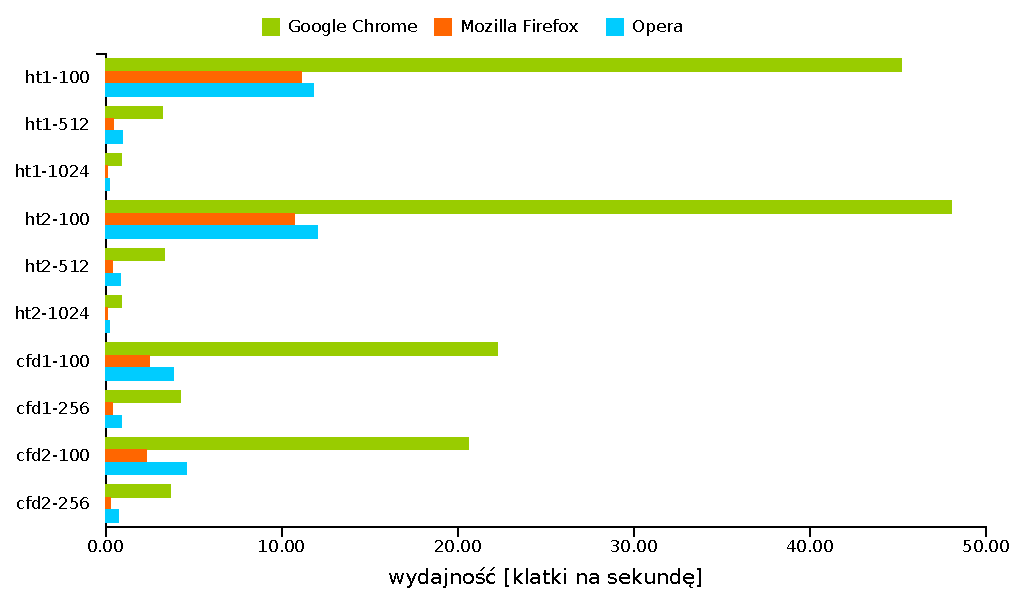
\includegraphics[width=\textwidth]{img/browserPerf}
\caption{Wydajność symulacji na CPU w zależności od przeglądarki}
\label{fig:browserPerf}
\end{figure}

\clearpage

\subsubsection{Obliczenia fizyczne wykonywane na GPU}

W przypadku symulacji, która obliczenia fizyczne przeprowadza na GPU, nie
została przetestowana Opera. Wynika to z faktu, iż w dniu kiedy testy były
przeprowadzane, wsparcie dla technologii \ow{WebGL} przez Operę nie było
wystarczające -- wyłącznie eksperymentalne w wyniku czego nie było
dostępu do niezbędnego rozszerzenia \ow{OES\_texture\_float}. Wyniki testów dla
przeglądarek Google Chrome oraz Mozilla Firefox przedstawiają tabela
\ref{tab:przegladarkiGPU} oraz wykres \ref{fig:browserPerfGPU}.

\begin{table}[!h]
\caption{Wydajność symulacji na GPU w zależności od przeglądarki}
\centering
\begin{tabular}{|c|p{3cm}|p{3cm}|}
\hline
test & Google Chrome & Mozilla Firefox \\ \hline
ht1-100 & 51.57 & 37.33 \\ \hline
h1-512 & 12.94 & 12.99 \\ \hline
ht1-1024 & 3.73 & 3.64 \\ \hline
ht2-100 & 48.84 & 37.59 \\ \hline
ht2-512 & 12.52 & 12.28 \\ \hline
ht2-1024 & 3.60 & 3.47 \\ \hline
cfd1-100 & 36.67 & 30.59 \\ \hline
cfd1-256 & 13.47 & 12.35 \\ \hline
cfd2-100 & 33.28 & 31.01 \\ \hline
cfd2-256 & 10.85 & 11.18 \\ \hline
\end{tabular}
\label{tab:przegladarkiGPU}
\end{table}

\begin{figure}[!h]
\centering
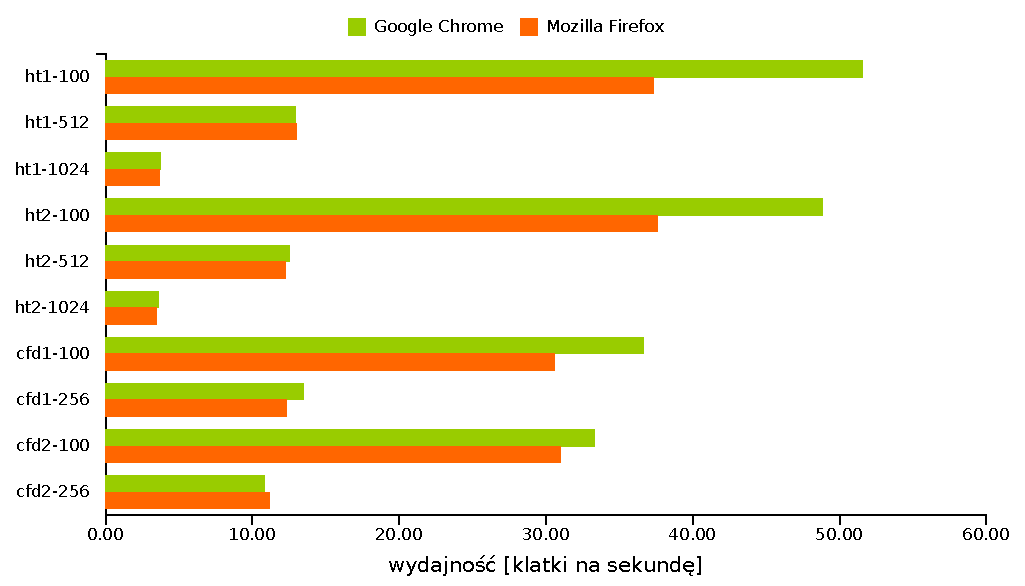
\includegraphics[width=0.9\textwidth]{img/browserPerfGPU}
\caption{Wydajność symulacji na GPU w zależności od przeglądarki}
\label{fig:browserPerfGPU}
\end{figure}

\clearpage

W przypadku obliczeń na GPU sytuacja diametralnie się zmienia. Różnice między
przeglądarkami, tak istotne przy obliczeniach na CPU, stają się znikome. Wynika
to z faktu, iż najbardziej obciążające obliczenia przeniesione są na kartę
graficzną i to jej wydajność jest decydująca, a nie wydajność silnika
\ow{JavaScript}. Potwierdza to fakt, iż przewagę Google Chrome widać wyłącznie
dla testów działających na najmniejszych siatkach. Są to jedyne przypadki, 
gdzie wydajność samego interpretera \ow{JavaScript} jest jeszcze istotna.

Innym ważnym wnioskiem jest to, iż użycie technologii \ow{WebGL} pozwala 
zniwelować różnice między wydjnością przeglądarek. O ile w przypadku obliczeń
na CPU jedynym rozsądnym środowiskiem wykonywania się symulacji była przeglądarka
Google Chrome, to przy zastosowaniu \ow{WebGL} możliwe staje się również użycie
Mozilli Firefox oraz każdej innej przeglądarki, która wspiera \ow{WebGL} (np.
Safari czy też w niedalekiej przyszłości także Opery).

\subsection{Analiza zysku wydajności wynikający z przeniesienia obliczeń na GPU}

\subsection{Wpływ optymalizacji i równoległości na jakość symulacji}

[TODO: rysunki, omówienie problemów z dokładniejszą siatką]

\section{Ocena dostępności aplikacji dla potencjalnych użytkowników}

\subsection{Wpływ posiadanej konfiguracji sprzętowej i oprogramowania na
symulator}

\section{Realizacja kluczowych wymagań}

\section{Podsumowanie}

	
\chapter{Wnioski}
	\section{Podsumowanie}
	\section{Dalszy rozwój}

%\chapter{Wprowadzenie}
\label{cha:wprowadzenie}

Większość ludzi w swoich domach i pracy może korzystać z dorobku technologicznej
rewolucji, która miała miejsce w ostatnich latach. Jednak w niektórych
dziedzinach życia zmiany następują znacznie wolniej - jedną z nich jest
edukacja. Komputery i internet stały się dostępne w większości szkół, jednak
programy i metody nauczania często nie nadążają za postępem technologicznym, są
wciąż reliktem poprzedniej epoki. Uczniowie pracują na komputerach najnowszej
generacji, jednak zwykle wykorzystują tylko ułamki ich możliwości, nie mając
dostępu do narzędzi, które faktycznie mogłyby przyczynić się do lepszego
zrozumienia poruszanych na lekcjach zagadnień. Najczęściej komputer i internet
stają się po prostu źródłem łatwo dostępnej wiedzy czy też miejscem gdzie pewne
problemy można próbować rozwiązywać wspólnie. Jest to oczywiście prawidłowe i
wartościowe wykorzystanie nowoczesnej technologi, ale jednocześnie też dosyć
powierzchowne i niewyczerpujące jej pełnych możliwości. Problemy i wyzwania
stojące przed współczesną edukacją szerzej porusza Andrew A. Zucker
\cite{Zuc2009}.

Edukacja może skorzystać na technologicznej rewolucji w znacznie większym
stopniu - jednym z pomysłów są wirtualne laboratoria, które pozwolą uczniom
eksplorować wybrane zagadnienia w sposób interaktywny, szczególnie podczas
nauczania przedmiotów ścisłych i przyrodniczych, tak istotnych w dzisiejszych
czasach. Cyfryzacja powinna zmienić tradycyjne oblicze lekcji z podręcznikiem i
zeszytem na pracę przy narzędziach edukacyjnych nowej generacji, wykorzystując
powszechną dostępność nowoczesnych technologii. Takie aplikacje również
doskonale wpisują się w popularną ideę cyfrowych podręczników. Dosłowne
przeniesienie zawartości papierowych książek na ekrany komputerów nie wiązałoby
się ze znaczącymi zmianami - inny byłby tylko nośnik słów, wiedzy. Bez zmian
natomiast pozostałby sam proces i metody uczenia przez uczniów i studentów.
Jednak jeśli wirtualny podręcznik zostanie zintegrowany z interaktywnymi
aplikacjami, pozwoli to zupełnie zmienić oblicze nauki. Uczeń będzie miał
możliwość prawdziwej eksploracji zagadnień, eksperymentowania we własnym domu,
przed własnym komputerem, podczas codziennej nauki, która może zamienić się w
prawdziwą, wartościową i przede wszystkim rozwijającą przygodę.

Najlepszym pomysłem dla podręczników przyszłości wydaje się umiejscowienie ich w
internecie. Dzięki dystrybucji poprzez to medium można uzyskać niezwykle łatwy i
powszechny dostęp, jako że połączenie z internetem jest w dzisiejszych czasach
czymś w pełni osiągalnym. Internetowa dystrybucja niesie również mnóstwo
korzyści nie tylko dla użytkowników podręczników, ale także dla ich twórców -
wystarczy wymienić zalety takie jak łatwość aktualizacji i docierania do
odbiorców. W związku z tym, również narzędzia stanowiące interaktywne elementy
podręczników przyszłości powinny być przystosowane do działania w środowisku
przeglądarki internetowej. Jest to zadanie wymagające, jednak niedawny rozwój
technologii i standardów internetowych takich jak HTML5 oraz WebGL, jak również
gwałtowne zmiany w samych przeglądarkach internetowych, dają ogromne możliwości
w tej materii.

Wymienione pomysły nie są tylko planami na przyszłość - te zmiany już powoli
następują, cyfrowe podręczniki i wirtualne laboratoria są trakcie rozwoju. Jedną
z organizacji zajmujących się wprowadzaniem najnowszych osiągnięć techniki do
szkół jest \mbox{The Concord Consortium}.

\section{Cel pracy}
\label{sec:celPracy}

W wyniku współpracy ze wspomnianą organizacją \mbox{The Concord Consortium}
powstał wydajny symulator fizyczny prezentujący zjawisko przewodnictwa cieplnego
oraz dynamikę płynów działający w środowisku przeglądarki internetowej o nazwie
\emph{\mbox{Energy2D}}. Ta interaktywna aplikacja doskonale wpisuje się w
przedstawioną ideę wirtualnych podręczników i laboratoriów, umożliwiając
użytkownikom łatwiejsze zrozumienie praw fizyki, które rządzą transferem
energii.

Celem niniejszej pracy jest przedstawienie rozwiązań, które umożliwiły powstanie
symulatora, ze szczególnym naciskiem na technologię WebGL, której niestandardowe
i nowatorskie zastosowanie pozwoliło zrównoleglić obliczenia fizyczne i tym
samym osiągnąć znaczący wzrost wydajności.

\section{Organizacja dokumentu}
\label{sec:organizacjaDokumentu}

Dalsze rozdziały przedstawiają kolejno:

\begin{itemize} \item Przedstawienie możliwości symulatora \en, wprowadzenie
do problematyki symulacji dynamiki płynów i przewodnictwa cieplnego oraz
przegląd istniejących, podobnych rozwiązań.

\item Opis podstawowej implementacji aplikacji, ze szczególnym uwzględnieniem
zagadnień związanych z jej architekturą i wnioskami, które można rozszerzyć na
ogół złożonych systemów \ow{JavaScript}.

\item Prezentację kluczowych technik dzięki którym udało się zrównoleglić
silniki fizyczne symulatora \en przy pomocy technologii \ow{WebGL}.

\item Ocenę systemu, w szczególności testy jakościowe, wydajnościowe oraz
badanie jak konfiguracja sprzętowa użytkownika wpływa na odbiór i jakość
symulacji.

\item Podsumowanie, wnioski, oraz pomysły na dalszy rozwój aplikacji.
\end{itemize}

%\chapter{Przeniesienie obliczeń fizycznych na procesor karty graficznej}

Niniejszy rozdział prezentuje techniki zastosowane w celu przeniesienia głównych
obliczeń fizycznych na kartę graficzną w symulatorze \ow{Energy2D} będącym
przedmiotem tej pracy. Na początku opisane są tradycyjne podejścia do tego
problemu dla aplikacji działających w natywnym środowisku systemu operacyjnego
oraz ich odniesienie do środowiska oferowanego przez przeglądarki internetowe.
Następnie zaprezentowane zostały najważniejsze zagadnienia dotyczące
implementacji równoległych silników fizycznych \ow{Energy2D} działających na
procesorze karty graficznej. Informacje te mogą być szczególnie użyteczne przy
próbach podobnych optymalizacji innych aplikacji.

Dzięki przeniesieniu obliczeń fizycznych na GPU uzyskano istotny wzrost
wydajności. Dokładna analiza zysków ze zrównoleglenia symulacji jest przedstawiona
w rozdziale \ref{cha:ocena}.

\section{Typowe metody przenoszenia obliczeń na GPU, a przeglądarka internetowa}

Współczesna karty graficzne posiadają ogromną moc obliczeniową -- wielokrotnie
większą od centralnego procesora przy założeniu, że obliczenia da się wykonywać
w sposób równoległy. Pomysł aby przenieść część obliczeń ogólnego zastosowania
na kartę graficzną pojawił się wraz z dynamicznym rozwojem procesorów
graficznych. Szczególnie istotnym momentem było wprowadzenie programowalnych
jednostek cieniujących (specyfikacja \ow{DirectX 8}). Dalszy rozwój obliczeń
ogólnego zastosowania na kartach graficznych (ang. \emph{General-Purpose
Computing on Graphics Processing Units}, w skrócie GPGPU) miał miejsce wraz z
wprowadzeniem technologii, które ukryły złożoność dostępu do zasobów karty
graficznej i udostępniły interfejs wysokiego poziomu. Wiodącymi technologiami
tego typu są \ow{OpenCL} (rozwiązanie otwarte) oraz \ow{CUDA} (zamknięte
rozwiązanie firmy NVIDIA, działające wyłącznie na sprzęcie tego producenta).

Wspomniane powyżej technologie dotyczą oczywiście aplikacji pisanych w natywnym
środowisku systemu operacyjnego. Aby programować jednostki cieniujące wystarczy
podstawowy dostęp do standardowego interfejsu \ow{OpenGL} bądź \ow{Direct3D}.
Implementacje tych interfejsów można znaleźć dla prawie każdego współczesnego
języka programowania. Interfejsy wyższego poziomu (\ow{OpenCL}, \ow{CUDA})
również posiadają implementacje w różnych językach programowania, choć
najczęstszym środowiskiem ich działania są aplikacje napisane w C bądź C++.

Poniżej krótko przedstawione są sposoby przeprowadzania obliczeń ogólnego
zastosowania na kartach graficznych oraz ich związek ze specyficznym
środowiskiem przeglądarki internetowej.

\subsection{Niskopoziomowe programowanie jednostek cieniujących}
\label{subsec:niskProgJedn}

Jest to najstarsze podejście do przeprowadzania obliczeń ogólnego zastosowania
na procesorze karty graficznej. Programista w swoisty sposób ,,oszukuje'' kartę
graficzną, przeprowadzając renderowanie prostej geometrii wyłącznie w celu
uruchomienia własnych programów jednostek cieniujących, które wykonują
obliczenia często nie mające nic wspólnego z generowaniem obrazu.

W przypadku technologii \ow{WebGL}, która posłużyła do zaimplementowania
silników fizycznych \en, diagram potoku renderowania prezentuje rysunek
\ref{fig:WebGLPipeline}. Zielonym kolorem zostały oznaczone procesy, które są
programowalne. Są to dwa rodzaje programów jednostek cieniujących --
wierzchołków oraz fragmentów. Nie ma możliwości bezpośredniego sterowania
pozostałymi procesami. Odbywają się one automatycznie, ewentualnie możliwa jest
konfiguracja pewnych parametrów. Dlatego też cały algorytm przeznaczony do
zrównoleglenia musi zostać zapisany wyłącznie przy użyciu programów wierzchołków
oraz fragmentów. Ponadto dane powinny się znajdować w pamięci karty graficznej,
najczęściej w postaci dwuwymiarowych tekstur.

\begin{figure}[!h]
\centering
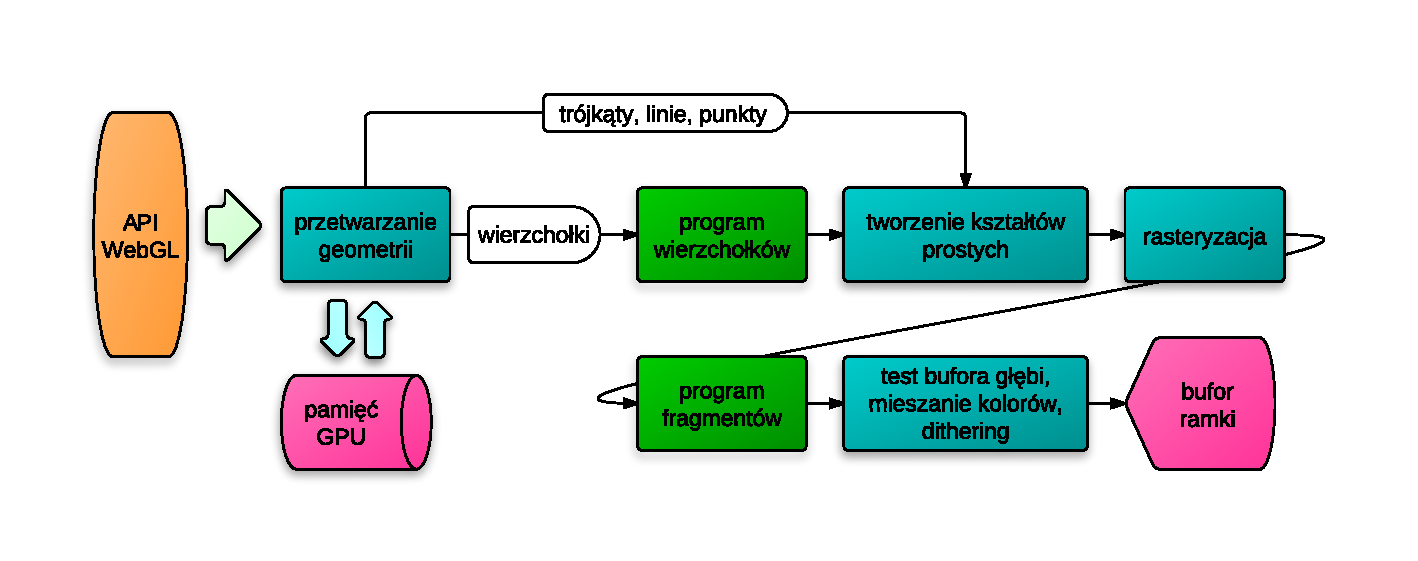
\includegraphics[width=\textwidth]{img/WebGLPipeline}
\caption{Diagram potoku renderowania \ow{WebGL} / \ow{OpenGL 3.x}}
\label{fig:WebGLPipeline}
\end{figure}

Takie podejście jednak jest wymagające i obarczone pewnymi problemami. Łatwo
popełnić błędy, wymagana jest też przynajmniej podstawowa wiedza o programowaniu
grafiki trójwymiarowej. Najważniejsze koncepcje niskopoziomowego programowania
jednostek cieniujących zostały doskonale przedstawione przez Marka Harrisa w
jednym z jego artykułów do popularnej serii \emph{GPU Gems} \cite{GPUConcepts}.

\subsection{Technologie wyższego poziomu}
\label{subsec:techWyzPoz}

Technologie, które przyczyniły się do gwałtownego wzrostu popularności obliczeń
na kartach graficznych to szczególnie \ow{OpenCL} oraz \ow{CUDA}.
Udostępniają  one znacznie wyższy poziom abstrakcji -- programista jest
zwolniony z obowiązku przyswojenia sobie niskopoziomowych mechanizmów rządzących
działaniem kart graficznych (choć ta wiedza pozwala tworzyć aplikacje
efektywniejsze). Udostępniony jest specjalny interfejs oraz składnia, co
znacznie ułatwia pracę, szczególnie programistom bez doświadczenia w pracy z
programowaniem grafiki trójwymiarowej.

\subsection{Możliwości w środowisku przeglądarki internetowej}
\label{subsec:srodPrzegInt}

Należy uściślić, że ,,środowisko przeglądarki internetowej'' to zbiór możliwości
nowoczesnych, wiodących przeglądarek internetowych, rozpowszechniony na tyle,
aby był dostępny dla większości użytkowników internetu. Równocześnie możliwości
te nie mogą wymagać instalowania żadnych dodatków i rozszerzeń, gdyż znacznie
ogranicza to ich dostępność. Jest to szczególnie istotne dla aplikacji
edukacyjnych, które wymagają łatwego i powszechnego dostępu.

Przeglądarka internetowa z założenia oferuje środowisko bardzo ograniczone,
przede wszystkim ze względów bezpieczeństwa. Jednak niedawno, wraz z nadejściem
standardu HTML5, został dodany podstawowy dostęp do zasobów karty graficznej.
Realizuje go technologia WebGL, która jest implementacją standardu \ow{OpenGL ES
2.0}. Tym samym pojawiła się możliwość programowania jednostek cieniujących kart
graficznych, a więc i przeprowadzania na nich obliczeń ogólnego zastosowania
(\ref{subsec:niskProgJedn}).

Technologie programowania kart graficznych wyższego poziomu
(\ref{subsec:techWyzPoz}) nie są (jeszcze) dostępne w przeglądarce internetowej.
Aktualnie trwają intensywne prace nad implementacją standardu OpenCL o roboczej
nazwie WebCL. Jednak technologia ta w aktualnym momencie jest na bardzo wczesnym
etapie rozwoju. Więcej informacji można znaleźć na stronie internetowej:
\url{http://www.khronos.org/webcl/}.

Dlatego też jedyną metodą na przeprowadzenie obliczeń ogólnego zastosowania na
procesorze karty graficznej w środowisku przeglądarki internetowej jest sposób
zaprezentowany w sekcji \ref{subsec:niskProgJedn}. Właśnie taka, niskopoziomowa
metoda została zastosowana dla silników fizycznych symulatora \ow{Energy2D}.
Opis najważniejszych zagadnień związanych z implementacją prezentuje następna
sekcja (\ref{sec:implSilFizWebGL}).

\section{Implementacji silników fizycznych Energy2D przy użyciu WebGL}
\label{sec:implSilFizWebGL}

Symulator \ow{Energy2D} składa się z dwóch kluczowych silników fizycznych -
przewodnictwa cieplnego oraz dynamiki płynów. Są one dokładnie przybliżone w
sekcji \ref{sec:silnikiFizyczne}. Oba te silniki są niezwykle wymagające
obliczeniowo. Dlatego też ich optymalizacja była zadaniem kluczowym, aby
stworzyć aplikację wartościową edukacyjnie. Zbyt wolny przebieg symulacji może
skutecznie zniechęcić większość potencjalnych użytkowników. Jednym z
podstawowych wymagań było, aby wirtualne laboratorium było aplikacją w pełni
interaktywną czyli również działającą jak najpłynniej.

Poniżej przedstawione są najważniejsze zagadnienia związanie z przeniesieniem
obliczeń fizycznych \ow{Energy2D} na kartę graficzną.

\subsection{Analiza algorytmów silników fizycznych pod kątem przetwarzania
równoległego}  

Wszystkie algorytmy rozwiązujące równania fizyczne w symulatorze \ow{Energy2D}
zostały poddane analizie pod kątem możliwości równoległego przetwarzania.
Zostały wyróżnione następujące kryteria, które algorytm musi spełniać, aby było
to możliwe:

\begin{itemize}

\item Możliwość reprezentowana danych w pamięci karty graficznej.

\item Niezależność wyniku algorytmu od sekwencji wykonywania obliczeń.

\end{itemize}

Jeżeli kryteria te są spełnione, powinna istnieć możliwość zaimplementowania
algorytmu w sposób równoległy. Oczywiście zmienia się strona techniczna, użyte
rozwiązania, język programowania oraz techniki, jednak sama koncepcja
algorytmu i główne kroki powinny pozostać bez większych zmian. Problem pojawia
się wtedy, gdy któryś z algorytmów nie spełnia jednego z tych kryteriów. W
takim przypadku konieczne są gruntowne modyfikacje lub rezygnacja z
implementacji takiego algorytmu.

Pierwszy warunek spełniają wszystkie algorytmy, jako że obliczenia są wykonywane
na prostokątnych siatkach symulacyjnych. Można je reprezentować w pamięci karty
graficznej przy użyciu dwuwymiarowych tekstur. Temat organizacji danych w
pamięci GPU oraz związane z tym problemy porusza sekcja \ref{sec:orgDanychWGPU}.

Drugi warunek nie został spełniony przez wszystkie zastosowane algorytmy.
Problematyczne okazały się metody rozwiązywania układów równań liniowych metodą
relaksacji \ow{Gaussa-Seidela} (por. \cite{GaussSeidel}). Podczas jednego
przebiegu przez wszystkie komórki macierzy, nowa wartość komórki $(i, j)$ jest
zależna od wartości komórek sąsiednich. Następnie komórka macierzy jest
niezwłocznie aktualizowana. Powoduje to, iż przy sekwencyjnym przetwarzaniu
wszystkich komórek, nowa wartość dla każdej komórki jest zależna od wartości
obliczonych zarówno w poprzednim kroku relaksacji jak i kroku aktualnym. W
sposób uproszczony schemat takiej relaksacji prezentuje algorytm
\ref{alg:GaussCPU}.

\begin{algorithm}[H]
  \caption{Relaksacja metodą Gaussa-Seidela na CPU}
  \label{alg:GaussCPU}
\begin{algorithmic}
\For {$0 \to relaxation\_steps$}
  \ForAll {$ \textrm{grid cells} $}
    \State $new\_val\gets f(x_{i,j}, x_{i+1,j}, x_{i-1,j}, x_{i,j+1}, x_{i,j-1})$
    \State $x_{i,j}\gets new\_val$
  \EndFor
\EndFor
\end{algorithmic}
\end{algorithm}

Niestety, przy obliczeniach równoległych nie można polegać na takiej zależności.
Każda komórka zostanie zaktualizowana na podstawie wartości komórek sąsiednich
wyłącznie z poprzedniego kroku relaksacji. Co więcej, ograniczeniem są też
kwestie czysto technologiczne - tekstury w których przechowywane są dane mogą
być podczas obliczeń wyłącznie przeznaczone do odczytu lub do zapisu. Tak więc
niemożliwy jest jednoczesny odczyt z danej tekstury oraz natychmiastowy zapis.

Problem ten został rozwiązany przez zmianę algorytmu rozwiązywania układów
równań liniowych na metodę relaksacji \ow{Jacobiego}. Główną różnicą jest moment
aktualizowania komórek siatki symulacji. W przeciwieństwie do metody \ow{Gaussa-
Seidela} nie następuje to natychmiast po obliczeniu nowej wartości dla danej
komórki, ale dopiero obliczeniu nowych wartości dla wszystkich komórek.
Uproszczony schemat tej relaksacji prezentuje algorytm \ref{alg:JacobiCPU}.

\begin{algorithm}[H]
  \caption{Relaksacja metodą Jacobiego na CPU}
  \label{alg:JacobiCPU}
\begin{algorithmic}
\For {$0 \to relaxation\_steps$}
  \ForAll {$ \textrm{grid cells} $}
    \State $temp_{i,j}\gets f(x_{i,j}, x_{i+1,j}, x_{i-1,j}, x_{i,j+1}, x_{i,j-1})$
  \EndFor
  \ForAll {$ \textrm{grid cells} $}
    \State $x_{i,j}\gets temp_{i,j}$
  \EndFor
\EndFor
\end{algorithmic}
\end{algorithm}

Taki algorytm można już przetworzyć na wersję równoległą. Macierze $x$ oraz
$temp$  zostają zamienione na odpowiednie tekstury. Również, w celach
wydajnościowych zawartość tekstur nie jest przepisywana tylko zamieniane są
ich referencje. Uproszczony schemat relaksacji metodą \ow{Jacobiego} na GPU
prezentuje algorytm \ref{alg:JacobiGPU}.

\begin{algorithm}[H]
  \caption{Relaksacja metodą Jacobiego na GPU}
  \label{alg:JacobiGPU}
\begin{algorithmic}
\For {$0 \to relaxation\_steps$}
  \ForAll {$ \textrm{grid cells} $} [IN PARALLEL]
    \State $temp_{i,j}\gets f(x_{i,j}, x_{i+1,j}, x_{i-1,j}, x_{i,j+1}, x_{i,j-1})$
  \EndFor
  \State swap $x$ with $temp$
\EndFor
\end{algorithmic}
\end{algorithm}

\begin{figure}[!p]
\centering

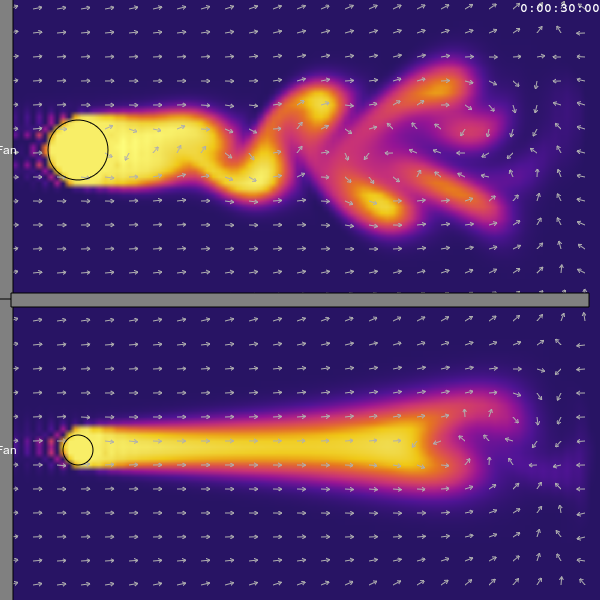
\includegraphics[width=.45\textwidth]{img/linSolvCPU5}
\caption{Symulacja przy użyciu metody Gaussa-Seidela na CPU, 
5 kroków relaksacji}
\label{fig:linSolvCPU5}

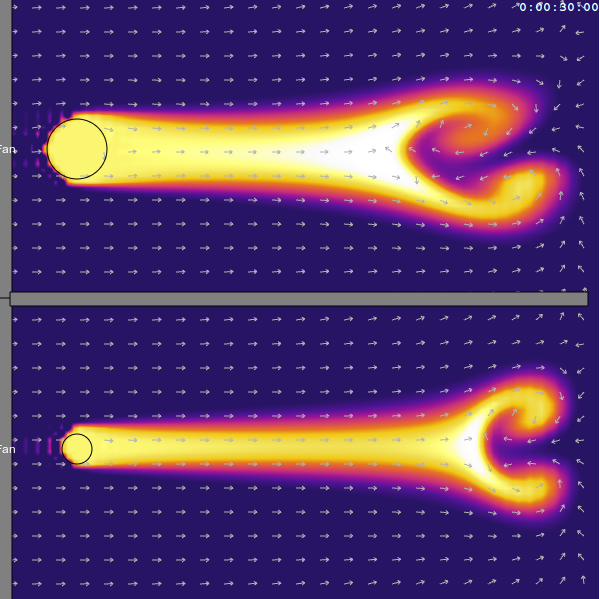
\includegraphics[width=.45\textwidth]{img/linSolvGPU5}
\caption{Symulacja przy użyciu metody Jacobiego na GPU, 
5 kroków relaksacji}
\label{fig:linSolvGPU5}

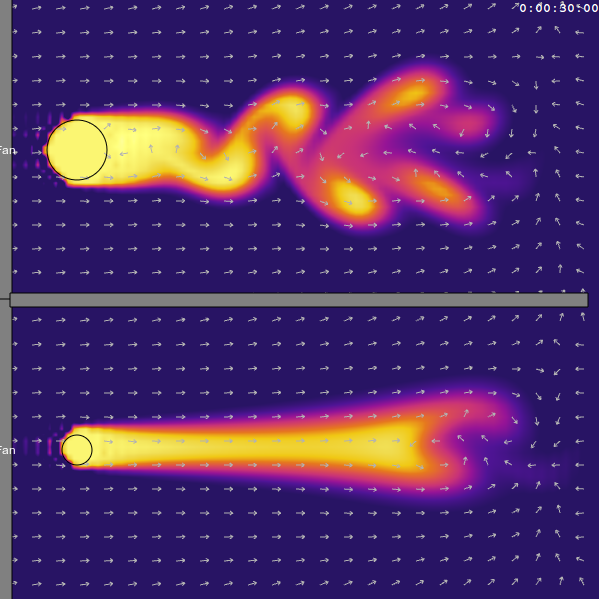
\includegraphics[width=.45\textwidth]{img/linSolvGPU10}
\caption{Symulacja przy użyciu metody Jacobiego na GPU, 
10 kroków relaksacji}
\label{fig:linSolvGPU10}

\end{figure}

Oczywiście zmiana algorytmu rozwiązywania równań liniowych niesie ze sobą
pewne konsekwencje. Inna jest konwergencja tych dwóch algorytmów. Metoda \ow
{Gaussa-Seidela} jest szybciej zbieżna niż metoda \ow{Jacobiego}. Efekty
symulacji dla różnej konfiguracji algorytmów rozwiązywania układów równań
liniowych prezentują rysunki \ref{fig:linSolvCPU5}, \ref{fig:linSolvGPU5} oraz
\ref{fig:linSolvGPU10}.

Na ww. rysunkach można zaobserwować wyraźne różnice w rezultatach symulacji. W
przypadku przedstawionej symulacji oczekiwanym wynikiem było powstane wiru
Kármána dla większej przeszkody. Przy implementacji równoległej metody
\ow{Jacobiego} widać, iż porządany efekt symulacji zostaje utracony. Dlatego
też należy wykonać więcej kroków relaksacji. Okazało się, że wartością
wystarczającą jest dziesięć. Wartość ta została ustalona empirycznie, tak aby
wyniki symulacji odpowiadały oczekiwaniom oraz były jak najbardziej zbliżone
do rezelutatów sekwencyjnych silików fizycznych. Jest to niezbędne, ponieważ
wersja równoległa aplikacji \en powinna być w pełni zgodnym i kompatybilnym
rozszerzeniem wersji podstawowej (sekwencyjnej, napisanej bez użycia
technologii \ow{WebGL}). Oczywiście wiąże się to ze spowolnieniem symulacji,
jednak w żadnym wypadku nie neguje opłacalności przeniesienia obliczeń na
kartę graficzną -- relaksacja na GPU jest wciąż dużo szybszych niż na CPU mimo
konieczności wykonania dwukrotnie większej liczby kroków.

Istnieją również implementacje algorytmu \ow{Gaussa-Seidela} na maszyny
równoległe. Nie są to dokładne kopie wersji sekwencyjnej, lecz imitują
obliczanie nowych wartości komórek na podstawie wartości z kroku relaksacji
poprzedniego i aktualnego. Doskonałe opracowanie zagadnień algorytmów
rozwiązujących układy równań liniowych na CPU oraz GPU, które okazało się
niezwykle przydatne podczas implementacji równoległych algorytmów dla \en,
zostało przygotowane przez G. Amadora oraz A. Gomesa \cite{LinSolvers}.
Niestety niskopoziomowa implementacja algorytmu \ow{Gaussa-Seidela} na GPU
wymaga wykonania dwóch procesów renderowania do tekstury dla jednego kroku
relaksacji -- powoduje to narzut czasowy, który w efekcie niweczy zysk z
szybszej konwergencji algorytmu.

\subsection{Podstawowy zarys implementacji}

Zgodnie z wnioskami sekcji \ref{subsec:srodPrzegInt}, ze względu na ograniczenia
środowiska przeglądarki internetowej, wymuszona została implementacja
niskopoziomowa przy użyciu technologii \ow{WebGL}. Opiera się ona na
programowaniu jednostek cieniujących karty graficznej, głównie wykorzystując
programy fragmentów (ang. fragment programs). Taka metoda przeprowadzania
obliczeń ogólnego przeznaczenia na karcie graficznej wymaga zrozumienia
podstawowych zagadnień związanych z programowaniem grafiki trójwymiarowej (por.
sekcja \ref{subsec:niskProgJedn}).

W przypadku implementacji \ow{Energy2D} podstawowy schemat przeprowadzania
obliczeń fizycznych na GPU z wykorzystaniem technologii \ow{WebGL} wygląda
następująco:

\begin{itemize}

\item Przygotowanie oraz kompilacja programów wierzchołków oraz fragmentów,
które zawierają implementację algorytmów silników fizycznych.

\item Przygotowanie tekstur, które przechowują dane symulacyjne. 

\item Przygotowanie danych geometrii płaszczyzny pokrywającej cały zakres
współrzędnych, które mieszczą się w obszarze renderowania.

\item Wykonywanie kolejnych kroków algorytmów fizycznych, co sprowadza się do:
	
	\begin{itemize}
	\item Renderowania wcześniej przygotowanej geometrii płaszczyzny przy użyciu
	wcześniej przygotowanych programów wierzchołków i fragmentów.

    \item Kopiowania danych z bufora ramki do wybranej tekstury przechowującej
	dane symulacji \footnote{Odbywa się to z użyciem obiektu bufora ramki (ang.
	FrameBuffer Object) z dołączoną do niego teksturą}.
	\end{itemize}

\end{itemize}

Poszczególne podpunkty w szerszym zakresie przybliżają sekcje od \ref{sec:progWierzFrag} do
\ref{sec:wykonNaGPU}.

\subsection{Programy wierzchołków oraz fragmentów}
\label{sec:progWierzFrag}

Właściwa implementacja algorytmów w programach wierzchołków i fragmentów
decyduje o poprawności oraz wydajności całej aplikacji. Bardzo często w
przypadku obliczeń ogólnego zastosowania na GPU, a także w przypadku
symulatora \ow{Energy2D}, większość pracy przypada na programy fragmentów.
Program wierzchołków zwykle sprowadza się do skopiowania wejściowych
współrzędnych wierzchołka i tekstury. Nie ma potrzeby jakiejkolwiek
modyfikacji geometrii renderowanej płaszczyzny. Dlatego też większość
programów wierzchołków w symulatorze Energy2D odpowiada poniższej
implementacji:

\begin{lstlisting}[language=GLSL, caption=Typowa implementacja programu
wierzchołków w symulatorze \ow{Energy2D} (język GLSL)]
attribute vec4 vertexPos;
attribute vec4 texCoord;

varying vec2 coord;
void main() {
  coord = texCoord;
  gl_Position = vertexPos;
}
\end{lstlisting}

Programy fragmentów, jako że wykonują właściwe obliczenia, nie są już tak
trywialne. Bardzo ważne jest właściwe określenie współrzędnych tekseli tekstury.
Posiadając siatkę symulacji o wymiarach NxN, należy ją zrzutować na zakres
domyślnych współrzędnych tekstury, które zawierają się w przedziale [0, 1].
Jeżeli zrobi się to nieprawidłowo, trudno będzie wykryć taki błąd, gdyż
domyślnie tekstury interpolują wartości leżące pomiędzy rzeczywistymi danymi.
Może to prowadzić do nieoczekiwanych rezultatów, stąd niezwykle istotne jest
precyzyjne określanie współrzędnych. W tym celu, praktycznie każdy program
fragmentów zawierał wektor o nazwie \ow{grid} równy (1.0 / N, 1.0 / N), gdzie
NxN to wymiary siatki symulacyjnej. Dodając lub odejmując odpowiedni jego
komponent można uzyskać dokładną wartość komórki sąsiedniej. Warto też pamiętać
o fakcie, iż pierwsza kolumna tekseli nie ma współrzędnej X równej 0.0, lecz 0.5
/ N. To samo dotyczy pierwszego rzędu współrzędnej Y równej 0.5 / N. Błędne
założenie, iż te kolumny mają współrzędne 0.0 prowadzi do problemów przy
wymuszaniu warunków brzegowych podczas symulacji. Ostatecznie, typowy szkielet
programów fragmentów wygląda następująco:

\begin{lstlisting}[language=GLSL, caption=Szkielet implementacji programu
fragmentów w symulatorze \ow{Energy2D} (język GLSL)]
uniform sampler2D simulationData;
uniform vec2 grid;
varying vec2 coord;

vec4 F(vec4 data) {
  // Funkcja wykonująca właściwe obliczenia dla danego kroku symulacji.
  // ...
}

void main() {
  vec4 data = texture2D(simulationData, coord);
  // Instrukcja warunkowa sprawdzająca czy nie są przetwarzane brzegi siatki.
  if (coord.x > grid.x && coord.x < 1.0 - grid.x &&
      coord.y > grid.y && coord.y < 1.0 - grid.y) {
    data = F(data);
  }
  gl_FragColor = data;
}
\end{lstlisting}

Oczywiście program, który wymuszał warunki brzegowe posiadał odwrotny warunek
w liniach 13 oraz 14. Implementacja funkcji $F$ nie jest przytoczona, gdyż nie
da się wyróżnić jakiegoś ogólnego jej schematu czy wzoru. Można powiedzieć, że
przenosząc dany krok algorytmu do języka GLSL, funkcja $F$ stanowi
implementację ,,wewnętrznych'' instrukcji zagnieżdżonych pętli iterujących po
wszystkich komórkach symulacji.


\subsection{Organizacja danych w pamięci karty graficznej}
\label{sec:orgDanychWGPU}
Dane symulacji (takie jak np. macierz temperatury czy macierz prędkości płynu)
przechowywane są w dwuwymiarowych teksturach zmiennoprzecinkowych. Tego typu
tekstury nie wchodzą w skład podstawowej specyfikacji \ow{WebGL 1.0}
(\cite{WebGLSpec}). W związku z tym wymagane jest użycie rozszerzenia
\ow{OES\_texture\_float}, które jest dostępne na większości
współczesnych urządzeń ([TODO: wspomnieć o rozdziale z testami]).

Niezwykle ważną kwestią jest organizacja danych w teksturze. Jest sporo
możliwości ponieważ tekstura z zasady nie jest wierną kopią tablicy JavaScript,
a obiektem przystosowanym do przechowywania obrazów (posiada na przykład kanały
kolorów). Dlatego też można rozważyć kilka potencjalnych sposobów na
rozmieszczenie danych.

\begin{itemize}

\item Schemat 1 -- tekstury jednokanałowe (format ALPHA lub LUMINANCE), jedna
tekstura odpowiada jednej tablicy JavaScript. Dalej nazywany schematem
\textbf{A1} na potrzeby niniejszego opracowania.

\item Schemat 2 -- tekstury czterokanałowe (format RGBA), dane tylko w jednym
kanale, jedna tekstura odpowiada jednej tablicy JavaScript. Dalej nazywany
schematem \textbf{RGBA1} na potrzeby niniejszego opracowania.

\item Schemat 3 -- tekstury czterokanałowe (format RGBA), dane w każdym z
kanałów, jedna tekstura odpowiada czterem tablicom JavaScript. Dalej nazywany
schematem \textbf{RGBA4} na potrzeby niniejszego opracowania.

\item Schemat 4 -- tekstury czterokanałowe (format RGBA), dane w każdym z
kanałów, jedna tekstura odpowiada jednej tablicy JavaScript, rozmiar tekstury
zredukowany czterokrotnie, gdyż każdy kanał odpowiada jednej ćwiartce tablicy.
Dalej nazywany schematem \textbf{RGBA1/4} na potrzeby niniejszego opracowania.

\end{itemize}

Każdy z powyższych schematów został przetestowany podczas implementacji
symulatora \ow{Energy2D}. Wyniki testów wydajnościowych przedstawia wykres
\ref{fig:texPerf}.

\begin{figure}[!h]
\centering
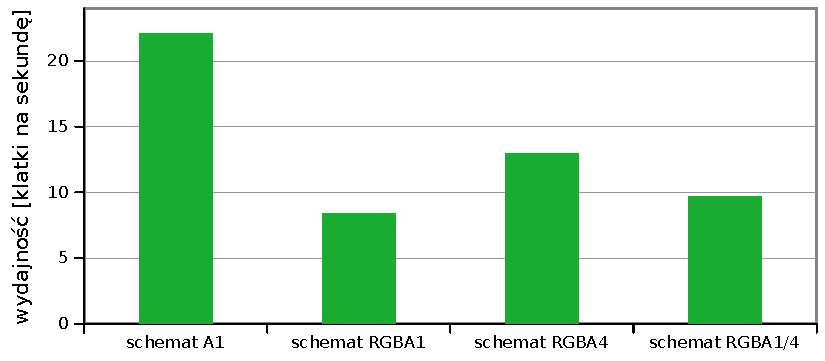
\includegraphics[width=.9\textwidth]{img/texPerf}
\caption{Wpływ organizacji danych w teksturach na wydajność symulacji 
\ow{Energy2D}}
\label{fig:texPerf}
\end{figure}

Rozwiązaniem optymalnym ze względu na wydajność oraz czytelność kodu wydaje się
schemat A1. Umożliwia on przeniesienie danych z tablic w relacji 1:1 do tekstur.
Do tego, każdy odczyt czy zapis do tekstury dotyczy tylko jednego kanału.
Niestety, na większości urządzeń nie ma możliwości dołączenia tekstury typu
ALPHA lub LUMINANCE do własnego obiektu bufora ramki (ang. FrameBuffer Object)
-- czyli renderowania do takiej tekstury \footnote{Testy zostały przeprowadzone
na systemie Linux (Ubuntu 12.04) i przeglądarce Google Chrome w wersji 22, która
korzysta z natywnego sterownika \ow{OpenGL}. Natomiast na tej samej konfiguracji
sprzętowej, ale działającej pod kontrolą systemu Windows nie udałoby się
uruchomić aplikacji. Podobnie w przypadku równie popularnego systemu
operacyjnego OS X.}. Wyklucza to możliwość użycia tego rozwiązania mimo
oczywistych zalet. Być może w przyszłości rozwój specyfikacji \ow{WebGL} na to
pozwoli.

Warto tutaj nadmienić, że specyfikacja \ow{WebGL} (\cite{WebGLSpec}) nie
gwarantuje, iż jakikolwiek z formatów tekstur zmiennoprzecinkowych będzie
zaakceptowany jako cel renderowania. Programista powinien wykonać test, aby
sprawdzić czy maszyna użytkownika wspiera daną konfigurację. Można to zrobić w
następujący sposób:

\begin{lstlisting}[language=JavaScript, caption=Weryfikacja poprawności formatu
i typu tekstury używanej jako cel renderowania]
var gl 		= getWebGLContext(),
	texture = gl.createTexture(),
	fbo 	= gl.createFramebuffer();

if (!gl.getExtension('OES_texture_float')) {
	throw new Error("Rozszerzenie OES_texture_float niedostępne.");
}
gl.bindTexture(gl.TEXTURE_2D, texture);
gl.texImage2D(gl.TEXTURE_2D, 0, gl.RGBA, 128, 128, 0, gl.RGBA, gl.FLOAT, null);
gl.bindFramebuffer(gl.FRAMEBUFFER, fbo);
gl.framebufferTexture2D(gl.FRAMEBUFFER, gl.COLOR_ATTACHMENT0, gl.TEXTURE_2D, texture, 0);
if (gl.checkFramebufferStatus(gl.FRAMEBUFFER) !== gl.FRAMEBUFFER_COMPLETE) {
	throw new Error("Dana tekstura nie jest wspierana jako cel renderowania.");
}
\end{lstlisting}

W praktyce tekstury zmiennoprzecinkowe posiadające cztery kanały kolorów są
najczęściej akceptowanym formatem do którego można zapisywać dane podczas
renderowania. Dlatego też schematy organizacji danych RGBA1, RGBA4 oraz RGBA1/4
używają takiego formatu tekstury.

Schemat RGBA1 posiada te same zalety co A1 jeśli chodzi o organizacje i
czytelność kodu źródłowego, jednak w tym przypadku dochodzi do dużego narzutu
wydajności związanego z odczytem i zapisem tekstur. Przy każdej z tych operacji
karta graficzna musi odczytać cztery kanały, jednak praktycznie wykorzystywany
jest tylko jeden z nich. Operacje dostępu do pamięci są czasochłonne, dlatego
też taka organizacja danych nie jest korzystna ze względów wydajnościowych.

Rozwiązaniem tego problemu są schematy RGBA4 oraz RGBA1/4. Organizacja danych
wg. trzeciego schematu pozwala zredukować narzut związany z odczytem oraz
zapisem pod warunkiem dobrej organizacji danych w teksturach. Pomysł ten
obrazuje diagram \ref{fig:rgba4Tex}. 

\begin{figure}[!h]
\centering
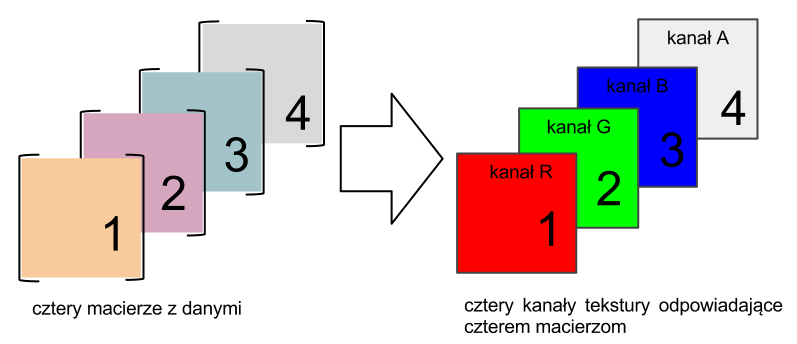
\includegraphics[width=.65\textwidth]{img/rgba4Tex}
\caption{Schemat organizacji danych z czterech macierzy w jednej teksturze}
\label{fig:rgba4Tex}
\end{figure}

Przy korzystnym ułożeniu danych jest możliwe praktycznie całkowite zredukowanie
narzutu związanego z odczytem wszystkich czterech kanałów tekstury, jednak w
praktyce jest to często niewykonalne. Przez korzystne rozmieszczenie danych
przyjmuje się takie ich ułożenie, żeby program jednostek cieniujących odczytując
teksturę faktycznie korzystał z danych zawartych w każdym z kanałów. Podobnie
przy zapisie, program renderujący powinien modyfikować wszystkie cztery kanały.
W przypadku symulatora \ow{Energy2D} udało się uzyskać taką organizację danych,
żeby odczyt był w znacznym stopniu zoptymalizowany, jednak podczas zapisu
modyfikowany był tylko jeden lub dwa kanały (kanał zawierający dane o
temperaturze lub kanały zawierające komponenty wektorów prędkości). Mimo nie do
końca optymalnego ułożenia kanałów, schemat RGBA4 okazał się wydajniejszy około
54\% od RGBA1.

\begin{figure}[!h]
\centering
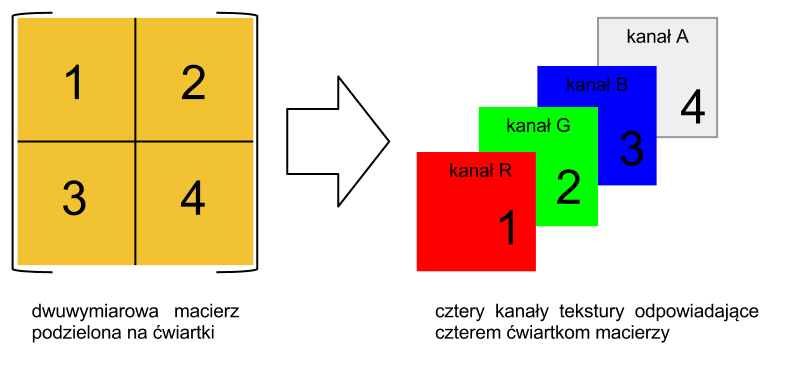
\includegraphics[width=.65\textwidth]{img/rgba14Tex}
\caption{Schemat organizacji danych macierzy NxN w teksturze (N/2)x(N/2)}
\label{fig:rgba14Tex}
\end{figure}

Ciekawą organizacją danych może wydawać się również pomysł przedstawiony w
schemacie RGBA1/4. Pozwala przechowywać tablicę JavaScript o wymiarach \ow{NxN}
w teksturze o wymiarach \ow{(N/2)x(N/2)}. Pomysł ten obrazuje diagram
\ref{fig:rgba14Tex}.

Taki układ danych teoretycznie posiada sporo zalet jak w przypadku użycia
tekstur jednokanałowych. Jednak znacznie zmniejsza on czytelność kodu i
komplikuje implementacje. Utrudnione zostaje przede wszystkim kontrolowanie
warunków brzegowych, programy jednostek cieniujących przetwarzają cztery pola
jednocześnie i stają się bardzo skomplikowane. W przypadku \ow{Energy2D}
komplikacje programów fragmentów były tak znaczne, że w efekcie odnotowano
bardzo słabe rezultaty pod względem wydajności. Symulacja okazała się być
wolniejsza około 34\% od symulacji korzystającej ze schematu RGBA4.

Dlatego też, ostatecznie w \ow{Energy2D} zastosowano schemat RGBA4. Zapewnia on
najlepszy kompromis pomiędzy dobrą wydajnością oraz wsparciem przez większość
dostępnych obecnie urządzeń.

\subsection{Geometria}

Podczas wykonywania obliczeń ogólnego przeznaczenia przy pomocy bezpośredniego
programowania jednostek cieniujących karty graficznej, niezbędne jest
stworzenie obiektu (a właściwie jego geometrii), który będzie renderowany. W
teorii może być to dowolna bryła. Jednak najczęściej pożądane jest, aby
program fragmentów wykonał się dla każdej komórki siatki symulacyjnej, którą
stanowi piksel tekstury. Można to osiągnąć renderując płaszczyznę, która
pokrywa całą dostępną przestrzeń renderowania.

Również w przypadku \en również wykorzystywany jest rendering takiej
płaszczyzny. Do przechowywania jej własności wykorzystane zostały bufory
wierzchołków (ang. vertex buffers) oraz indeksów (ang. index buffers)
znajdujące się w pamięci karty graficznej. Dzięki temu, podczas wielokrotnego
renderowania tej samej płaszczyzny, nie jest konieczne nieustanne przesyłanie
atrybutów wierzchołków do pamięci GPU.

W finalnej implementacji \en zostały przygotowane klasy pomocnicze
zarządzające geometrią oraz buforami. Jednak najprostszy sposób na stworzenie
płaszczyzny pokrywającej cały obszar renderowania oraz umieszczenie jej
atrybutów w pamięci karty graficznej zaprezentowany jest poniżej:

\begin{lstlisting}[language=JavaScript, caption=Definicja geometrii
płaszczyzny pokrywającej cały obszar renderowania]
var gl           = getWebGLContext(),
    vertexBuffer = gl.createBuffer(),
    indexBuffer  = gl.createBuffer(),
    vertexData,
    indexData;

// Współrzędne wierzchołków.
vertexData = new Float32Array([
    -1, -1, 
     1, -1,
    -1,  1,
     1,  1
]);
// Transfer do bufora wierzchołków.
gl.bindBuffer(gl.ARRAY_BUFFER, vertexBuffer);
gl.bufferData(gl.ARRAY_BUFFER, vertexData, gl.STATIC_DRAW);
// Indeksy trojkątów płaszczyzny.
indexData = new Uint16Array([
    0, 1, 2,
    2, 1, 3
]);
// Transfer do bufora indeksów.
gl.bindBuffer(gl.ELEMENT_ARRAY_BUFFER, indexBuffer);
gl.bufferData(gl.ELEMENT_ARRAY_BUFFER, indexData, gl.STATIC_DRAW);
\end{lstlisting}

\subsection{Wykonywanie kroków algorytmów na GPU}
\label{sec:wykonNaGPU}

Dysponując skompilowanymi programami wierzchołków oraz fragmentów, danymi
symulacji zapisanymi w teksturach dwuwymiarowych oraz niezbędną geometrią,
można przejść do faktycznej realizacji kroków algorytmów
zapisanych w programach jednostek cieniujących.

W przypadku technologii WebGL narzuca się schemat związany z techniką
renderowania do tekstury przy użyciu obiektu bufora ramki (ang. \emph{Frame
Buffer Object}). Związanie takiego obiektu z wybraną teksturą, a następnie
uaktywnienie przed właściwym renderowaniem, powoduje iż karta graficzna
automatycznie kopiuje zawartość bufora ramki do tekstury po zakończonym
renderowaniu.

Technika ta ma jednak kilka ograniczeń. Tekstura związana z obiektem bufora
ramki (czyli przeznaczona do zapisu) nie może być używana jednocześnie do
odczytu wartości. W związku z tym zawsze trzeba używać minimalnie jednej
tekstury tymczasowej. Następnie należy kopiować jej zawartość do tekstury
docelowej lub podmienić referencje. Oczywiście modyfikacja wyłącznie
referencji  jest znacznie efektywniejsza przez co i częściej stosowana.
Całościowo taki schemat nazywany jest ,,ping-pong rendering''.

Implementacja w języku \ow{JavaScript} przy użyciu technologi \ow{WebGL} nie
odbiega znacząco od implementacji w innych językach przy użyciu
,,tradycyjnego'' API OpenGL. Mark Harris zaprezentował najważniejsze aspekty
tej techniki w swoich artykułach opublikowanych w serii \emph{GPU Gems}
(\cite{GPUConcepts} oraz \cite{GPUFluid}).



% itd.
% \appendix
% \include{dodatekA}
% \include{dodatekB}
% itd.

\bibliographystyle{alpha}
\bibliography{bibliografia}

\end{document}
